%\document class[]{aiaa-tc} %load in aiaa class template file
\documentclass{article}
\usepackage{amsmath}
\usepackage{mathrsfs}
\usepackage{enumitem}
\usepackage{mathabx}
\usepackage{hyperref}
\usepackage{natbib} %REMOVE THIS IF YOU DON'T WANT BRACKETS ON YOUR PAPER
\usepackage{float}
\usepackage{color,soul}
\usepackage[font=normalsize,labelfont=bf]{caption}
\usepackage[left=2cm,right=2cm,top=2cm,bottom=2cm]{geometry}
\usepackage{graphicx}

\newcommand{\sref}[1]{$^{[\ref{#1}]}$}
\newcommand{\dref}[2]{$^{[\ref{#1}-\ref{#2}]}$}

 % Define commands to assure consistent treatment throughout document
\newcommand{\eqnref}[1]{(\ref{#1})}
\newcommand{\class}[1]{\texttt{#1}}
\newcommand{\package}[1]{\texttt{#1}}
\newcommand{\file}[1]{\texttt{#1}}
\newcommand{\BibTeX}{\textsc{Bib}\TeX}

\begin{document}

\begin{center}
\begin{LARGE}{\bf SpaceFlight Mechanics and Controls}\end{LARGE}\\
\large
\vspace{22 mm}
   A Brief Textbook Presented to the \\ 
   Student Body of the University of South Alabama \\
\vspace{22 mm}
%%by\\
\vspace{22 mm}
  %%Carlos Montalvo \\
\vspace{22 mm}
       %%{\itshape University of South Alabama}\\
       Last Update: \today\\
{\bf Copyright $\copyright$ Carlos Jos\'{e} Montalvo}
\end{center}

%%  \title{\bf Guidance Navigation and Control for Small Sats}

%%  \author{Carlos Montalvo\thanks{Assistant Professor, Department of Mechanical
%%     Engineering, cmontalvo@southalabama.edu}\\
%%    {\normalsize\itshape Facility for Aerospace Systems and Technology
%%      (FAST)}\\
%%    {\normalsize\itshape College of Engineering, University of South Alabama}\\
%%    {\normalsize\itshape 150 Jaguar Dr.}\\
%%    {\normalsize\itshape Shelby Hall Rm. 3125}\\
%% {\normalsize\itshape    Mobile, AL USA, 36688}\\}
%%  \date{}

\linespread{1}

\newpage

%% \begin{document}

%% \maketitle

\begin{abstract}

A CubeSAT is a small satellite on the order of 10 centimeters along
each axis. A 1U satellite is a small cube with 10 cm sides. These
satellites are used for a variety of missions and created by a variety
of different organizations. When deployed from 
a rocket, a CubeSAT may obtain a large angular velocity
which must be reduced before most science missions or communications
can take place. Maximizing solar energy charging also involves
better pointing accuracy. To control the attitude of these small
satellites, reaction wheels, magnetorquers and even the gravity
gradient are used in low earth orbit (LEO) while reaction control thrusters
are typically used in deep space.  On a standard LEO CubeSAT, 3 reaction
wheels are used as well as 3 magnetorquers. In the initial phase of
the CubeSAT mission, the magnetorquers are used to reduce the angular
velocity of the satellite down to a manageable level. Once the norm of the angular velocity is
low enough, the reaction wheels can spin up reducing the angular
velocity to zero. At this point a Sun finding algorithm is employed to
find the Sun and fully charge the batteries. In LEO two independent
vectors are obtained, the Sun vector and the magnetic field vector, to
determine the current attitude of the vehicle which is typically
called attitude determination. Other sensors such as horizon sensors,
star trackers and even lunar sensors can be used to obtain the
quaternion of the vehicle. This paper investigates the necessary
mathematics to understand the intricacies of guidance, navigation and
control specifically discussing the attitude determination and
controls subsystem (ADACS). 

\end{abstract}

%%%%%%%%%%%%%%%%%%%%%%%%%%%%%%%%%%%%%%%%%%%%%%%%%%%%%%%%%%%%%%%%%%%
%%%%%%%%%%%%%%%%%%%%%%%%%%%%%%%%%%%%%%%%%%%%%%%%%%%%%%%%%%%%%%%%%%%
%%%%%%%%%%%%%%%%%%%%%%%%%%%%%%%%%%%%%%%%%%%%%%%%%%%%%%%%%%%%%%%%%%%

\begin{tabbing}
  XXXXXXXXXX \= \kill% this line sets tab stop
  $x,y,z$ \> components of the mass center position vector in the
  inertial frame (m)  \\
  $\phi,\theta,\psi$ \> Euler roll,pitch, and yaw angles (rad) \\
  $q_0,q_1,q_2,q_3$ \>  quaternions \\  
  $u,v,w$ \> components of the mass center velocity vector in the
  body frame (m/s)  \\
  $p,q,r$ \> components of the mass center angular velocity vector in the
  body frame (rad/s)  \\
  $\vec{\omega}_{B/I}$ \> angular velocity vector of the satellite in
  the body frame (rad/s) \\
  ${\bf T}_{IB}$ \> rotation matrix from frame I to frame B \\
  ${\bf H}$ \> relationship between angular velocity components in
  body frame and derivative of Euler angles \\
  $m$ \> mass (kg) \\
  $I$ \> mass moment inertia matrix about the mass center
  in the body frame ($kg-m^2$)  \\
  $X,Y,Z$ \> components of the total force applied to CubeSAT in
  body frame (N)  \\
  $L,M,N$ \> components of the total moment applied to CubeSAT in
  body frame (N-m)  \\
  ${\vec r}_{A\rightarrow B}$ \> position vector from a generic point A
  to a generic point B (m) \\
  ${\vec V}_{A/B}$ \> velocity vector of a generic point A
  with respect to a generic frame B (m/s) \\
  ${\bf S}(\vec{r})$ \> skew symmetric matrix operator on a
  vector. Multiplying this matrix by a vector is equivalent \\
  \> to a cross product\\
\end{tabbing}

\newpage

\section*{Manuscript Changes}

\begin{enumerate}[itemsep=-5pt]
\item June 10th, 2020 - Magnetic Field Model section updated to
  reflect the difference between the East North Vertical and the North
  East Down reference frames. The Figure showing the magnetic field
  for an example Low Earth Orbit has also been update. Also added this
  page for manuscript changes and the following pages that list where
  this file can be found.
\item December 10th, 2020 - Moved to public Github Repo separate from MATLAB
\end{enumerate}

\newpage

\section*{Changes Needed}

\begin{enumerate}[itemsep=-5pt]
\item Need to add derivation of a complimentary filter using
  transfer functions which means I probably need to add in transfer
  functions into this manuscript
\item Need to make Orbital Elements its own section. Discuss how to
  get position and velocity from orbital elements and orbital elements
  from position and velocity.
\item Need to explain the difference between Geodetic and Geocentric
  coordinates
\item Need to add the computation of latitude an longitude from
  cartesian and vice versa as well as flat Earth approximation
\item Derivation of ground path taking into account orbital
  precession, rotation of the Earth and swath angle from projection of
  a satellite onto the Earth. See pdf from the Air Force. A Google
  search will hopefully turn up the paper I'm thinking of.
\end{enumerate}

\newpage

\section*{Current Distribution List of Manuscript}
\begin{enumerate}[itemsep=-5pt]
\item Main Document Location\url{https://github.com/cmontalvo251/MATLAB.git/Space_Flight_Mechanics_Montalvo} - This is a public
  repository on Github for everyone to download.
\end{enumerate}
  
\newpage

\tableofcontents

\newpage

%%%%%%%%%%%%%%%%%%%%%%%%%%%%%%%%%%%%%%%%%%%%%%%%%%%%%%%%%%%%%%%%%%%
%%%%%%%%%%%%%%%%%%%%%%%%%%%%%%%%%%%%%%%%%%%%%%%%%%%%%%%%%%%%%%%%%%%
%%%%%%%%%%%%%%%%%%%%%%%%%%%%%%%%%%%%%%%%%%%%%%%%%%%%%%%%%%%%%%%%%%%

\section{Particle Dynamics}

\subsection{Systems of Particles}

For this formulation we start with Newton's Second Law with no
approximations. Similar dynamic forumlations can be found in \cite{etkins,
  phillips,nelson,astrodynamics}.
\begin{equation}
\sum\limits_{i=0}^N \vec{F}_{ji} = \frac{d\vec{p}_j}{dt}
\end{equation}
where $\vec{p}_j$ is the momentum of a particle. $\vec{F}_{ji}$ is a
force on the particle. The statement above states that sum of all
forces on a particle is equal to the time rate of change of
momentum. If two particles are then considered the equation can
be written for both particles.
\begin{equation}
\begin{matrix}
\sum\limits_{i=0}^N \vec{F}_{1i} + \vec{f}_{12} = \frac{d\vec{p}_1}{dt} &
\sum\limits_{i=0}^N \vec{F}_{2i} + \vec{f}_{21} = \frac{d\vec{p}_2}{dt} 
\end{matrix}
\end{equation}
Note that the forces $\vec{f}_{12}$ and $\vec{f}_{21}$ are internal forces
experienced by each particle exerted on each other since they are
rigidly connected. Newton's Third Law states that for every action
there is an equal and opposite reaction. That is, $\vec{f}_{12} = -\vec{f}_{21}$. Thus, if both equations are added the following equation is
created
\begin{equation}
\sum\limits_{j=0}^P \sum\limits_{i=0}^N \vec{F}_{ji} =
\sum\limits_{j=0}^P \frac{d\vec{p}_j}{dt}
\end{equation}
where P is the number of particles. Typically the double summation
in F is written just as $\vec{F}$.

\subsection{Rotational Dynamics for Systems of Particles}

Note that by construction, a system of particles rigidly connected can
now rotate about a center point. The center of mass of a system of
particles can be defined using the relationship below
\begin{equation}
\vec{r}_C = \frac{1}{m}\sum\limits_{j=0}^P m_j\vec{r}_{j}
\end{equation}
where
\begin{equation}
m = \sum\limits_{j=0}^P m_j
\end{equation}
This vector can then be used to create rotational dynamics starting
with the linear dynamics.
\begin{equation}
\sum\limits_{j=0}^P \sum\limits_{i=0}^N {\bf S}(\vec{r}_{Cj}) \vec{F}_{ji}  = \vec{M}_C = \sum\limits_{j=0}^P {\bf
  S}(\vec{r}_{Cj}) \frac{d\vec{p}_j}{dt}
\end{equation}
where ${\bf S}(\vec{r}_{Cj})$ is the skew symmetric matrix of the
vector from the center of mass to the jth particle which results in a
cross product. The skew symmetric operator is denoted by ${\bf
  S}()$. 
\begin{equation}
{\bf S}(\vec{r}_{Cj}) = \begin{bmatrix} 0 & -z_{Cj} & y_{Cj} \\ z_{Cj} & 0 &
  -x_{Cj} \\ -y_{Cj} & x_{Cj} & 0 \end{bmatrix}
\end{equation}
\section{Rigid Bodies}
At this point, many assumptions are made about the
system of particles.
\begin{enumerate}
\item The mass of each particle or rigid body is constant.
\item An inertial frame is placed at the center of the Earth that does
  not rotate with the Earth. We assume that the Earth is ``fixed" to
  this point but still rotates. The coordinates of our satellite
  though are expressed in this non-rotating inertial frame. This is
  explained in more detail later.
\item The rigid body is not flexible and does not change shape. That
  is, the time rate of change of the magnitude of a vector
  $\vec{r}_{PQ}$ is zero for any arbitrary points P and Q attached to
  the rigid body.
\end{enumerate}

\subsection{Translational Dynamics}

Using all of these simplifications, the momentum term on the right can
be simplified to 
\begin{equation}
\sum\limits_{j=0}^P \vec{p}_j = m \vec{v}_{C/I}
\end{equation}
The derivation of the term above starts by deriving the position of
the center of mass as the following equation.
\begin{equation}
\vec{r}_{j} = \vec{r}_C + \vec{r}_{Cj}
\end{equation}
Taking one derivative results in the following equation
\begin{equation}
\vec{v}_{j/I} = \vec{v}_{C/I} + \frac{{}^Bd \vec{r}_{Cj}}{dt} +
{\bf S}(\vec{\omega}_{B/I}) \vec{r}_{Cj}
\end{equation}
where ${\bf S}(\vec{\omega}_{B/I})$ is the skew symmetric matrix of the
angular velocity vector which results in a cross product. This
equation comes from the derivative transport theorem. Since the body
is a rigid body the term $\frac{{}^Bd \vec{r}_{Cj}}{dt}=0$ resulting
in the equation below
\begin{equation}
\vec{v}_{j/I} = \vec{v}_{C/I} + {\bf S}(\vec{\omega}_{B/I}) \vec{r}_{Cj}
\end{equation}
which any dynamicist knows as the equation for two points fixed on a
rigid body. This equation can then be substituted into the equation
for momentum such that.
\begin{equation}
\sum\limits_{j=0}^P \vec{p}_j =  \sum\limits_{j=0}^P m_j \left(\vec{v}_{C/I}
+ {\bf S}(\vec{\omega}_{B/I}) \vec{r}_{Cj}\right)
\end{equation}
The first term reduces to 
\begin{equation}
\sum\limits_{j=0}^P m_j \vec{v}_{C/I} =  \vec{v}_{C/I}
\sum\limits_{j=0}^P m_j =  m \vec{v}_{C/I} 
\end{equation}
the second term reduces to zero since the sum of all particles from
the center of mass is by definition the center of mass and thus zero.
\begin{equation}
\sum\limits_{j=0}^P {\bf S}(\vec{\omega}_{B/I}) m_j\vec{r}_{Cj} =
{\bf S}(\vec{\omega}_{B/I})\sum\limits_{j=0}^P m_j\vec{r}_{Cj} = 0
\end{equation}
Plugging this result for momentum into Newton's equation of motion
yields. This is typically called Newton-Euler equations of motion.
\begin{equation}
\vec{F}_C = m \left(\frac{{}^Bd \vec{v}_{C/I}}{dt} +
{\bf S}(\vec{\omega})_{B/I} \vec{v}_{C/I} \right)
\end{equation}

\subsection{Rotational Dynamics}

Plugging in the expression for two points fixed on a rigid body
results in a much different expression. First let's expand the
rotational dynamic equations of particles using the assumptions made
for a rigid body.
\begin{equation}
\vec{M}_C = \frac{d}{dt}\sum\limits_{j=0}^P {\bf S}(\vec{r}_{Cj}) m_j\vec{v}_{j/I}
\end{equation}
Then the equation of two points fixed on a rigid body can be
introduced to obtain the following equation
\begin{equation}
\vec{M}_C = \frac{d}{dt}\sum\limits_{j=0}^P {\bf S}(\vec{r}_{Cj}) m_j\left(\vec{v}_{C/I} + {\bf S}(\vec{\omega}_{B/I}) \vec{r}_{Cj}\right)
\end{equation}
expanding this into two terms yields
\begin{equation}
\vec{M}_C =  \frac{d}{dt}\left(\sum\limits_{j=0}^P m_j{\bf S}(\vec{r}_{Cj}) {\bf S}(\vec{\omega}_{B/I}) \vec{r}_{Cj} + \sum\limits_{j=0}^P {\bf S}(\vec{r}_{Cj})m_j\vec{v}_{C/I}\right)
\end{equation}
To simplify this further a useful equality is used for cross
products. That is ${\bf S}(\vec{a})\vec{b}=-{\bf
  S}(\vec{b})\vec{a}$. The equation above then changes to
\begin{equation}
\vec{M}_C =  \frac{d}{dt}\left(\left(-\sum\limits_{j=0}^P m_j{\bf S}(\vec{r}_{Cj}){\bf
  S}(\vec{r}_{Cj})\right)\vec{\omega}_{B/I} - {\bf S}(\vec{v}_{C/I})
\sum\limits_{j=0}^P \vec{r}_{Cj}m_j\right)
\end{equation}
Notice, that parentheses were placed around the first term to isolate
the angular velocity. This is because the angular velocity is constant
across the system of particles. The term on the right has also been
altered slightly to isolate the fact that the velocity of the center
of mass is independent of the system of particles. With the equation
in this form it is easy to see that the term on the right is zero
because it is the definition of the center of mass. The equation then
reduces to 
\begin{equation}
\vec{M}_C =  \frac{d}{dt}\left(\sum\limits_{j=0}^P m_j{\bf S}(\vec{r}_{Cj}){\bf
  S}(\vec{r}_{Cj})^T\right)\vec{\omega}_{B/I} 
\end{equation}
Notice again that minus sign has been removed. The skew symmetric
matrix has an interesting property where the transpose is equal to the
negative of the original matrix. The term in brackets is a well known
value for rigid bodies and is known as the moment of inertia for rigid
bodies. 
\begin{equation}
{\bf I}_C =  \sum\limits_{j=0}^P m_j{\bf S}(\vec{r}_{Cj}){\bf
  S}(\vec{r}_{Cj})^T
\end{equation}
This results in the kinematic equations of motion for rigid bodies to
the simple equation below.
\begin{equation}
\vec{M}_C =  \frac{d}{dt}\left({\bf I}_C\vec{\omega}_{B/I} \right)
\end{equation}
With the equation in this form it is finally possible to carry out the
derivative
\begin{equation}
\vec{M}_C = \frac{{}^Bd ({\bf I}_C\vec{\omega}_{B/I})}{dt} + {\bf
  S}(\vec{\omega}_{B/I}){\bf I}_C\vec{\omega}_{B/I}
\end{equation}
The first term requires the chain rule to perform the derivative and
can thus result in a time varying moment of inertia matrix and the
derivative of angular velocity. Therefore the equation can simply be written as
\begin{equation}
\vec{M}_C = \dot{{\bf I}}\vec{\omega}_{B/I} + {\bf I}_C\frac{{}^Bd (\vec{\omega}_{B/I})}{dt} + {\bf
  S}(\vec{\omega}_{B/I}){\bf I}_C\vec{\omega}_{B/I}
\end{equation}

\section{Attitude Parameterization of Rigid Bodies}

\subsection{Euler Angles}\label{s:Euler_Angles}

\subsubsection{General 3-2-1 Sequence}

It is possible to obtain the orientation of a satellite using Euler
angles. This is constructed using the standard aircraft flight mechanics rotation
sequence (3-2-1) where a yaw $\psi$ rotation is done along the z-axis,
a pitch $\theta$ rotation is done about the intermediate y-axis and
then a final rotation about the x-axis through roll $\phi$ is
done. A Figure of this is shown below.
\begin{figure}[H]
  \begin{center}
  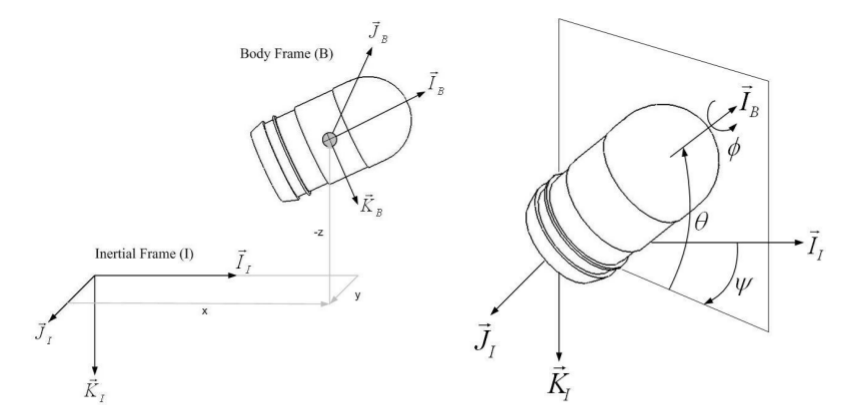
\includegraphics[height=50mm, width=120mm]{Figures/6DOFrocketschematic.png}
  \end{center}
  \caption{Six Degree of Freedom Schematic}
\end{figure}
Putting all of these 2-D rotations together creates a
transformation matrix from body to inertial. Standard shorthand
notation is used for trigonometric functions: $ cos(\alpha) \equiv
c_{\alpha} $ , $ sin(\alpha) \equiv s_{\alpha} $ , and $ tan(\alpha)
\equiv t_{\alpha} $.
\begin{equation}\label{e:TIB}
{\bf T}_{IB}(\phi,\theta,\psi) = \begin{bmatrix} c_{\theta}c_{\psi} &
s_{\phi}s_{\theta}c_{\psi}-c_{\phi}s_{\psi} &
c_{\phi}s_{\theta}c_{\psi} + s_{\phi}s_{\psi} \\ c_{\theta}s_{\psi} &
s_{\phi}s_{\theta}s_{\psi} + c_{\phi}c_{\psi} &
c_{\phi}s_{\theta}s_{\psi} - s_{\phi}c_{\psi} \\
-s_{\theta} & s_{\phi}c_{\theta} & c_{\phi}c_{\theta}
\end{bmatrix}
\end{equation}

\subsubsection{Derivatives}

If Euler angles are used to parameterize the orientation, the
derivative of Euler angles is somewhat cumbersome to obtain. The angular
velocity of a body is typically written as
\begin{equation}
\vec{\omega}_{B/I} = \begin{Bmatrix} p \\ q
  \\ r \end{Bmatrix} = p \hat{I}_B + q \hat{J}_B + r \hat{K}_B
\end{equation}
There are no inertial components for the angular velocity
vector. However, a relationship can be derived relating the
derivatives of the Euler angles. The angular velocity can be written
in vector form such that
\begin{equation}
\vec{\omega}_{B/I} = \dot{\psi} \hat{K}_I + \dot{\theta} \hat{J}_{NR} +
\dot{\phi} \hat{I}_B
\end{equation}
relating the unit vectors $\hat{K}_I$ and $\hat{J}_{NR}$ to the body
frame using the planar rotation matrices results in the equation
below. Note that NR is denoted as the ``No-Roll" frame.
\begin{equation}\label{e:ptpdot}
\begin{Bmatrix} \dot{\phi} \\ \dot{\theta} \\ \dot{\psi} \end{Bmatrix}
= [\textbf{H}]
\begin{Bmatrix} p\\q\\r\end{Bmatrix}
\end{equation}
where
\begin{equation}
\textbf{H}=\begin{bmatrix} 1 & s_{\phi}t_{\theta} & c_{\phi}t_{\theta} \\ 0 &
c_{\phi} & -s_{\phi} \\ 0 & s_{\phi}/c_{\theta} &
c_{\phi}/c_{\theta} \end{bmatrix}
\end{equation}

\subsubsection{Screw Rotation}

It is often useful to extract Euler Angles from a unit vector. A unit
vector has two degrees of freedom and thus has two rotations
$\psi$ and $\theta$ which can be determined using the
equation below where $\hat{n}(1)$ denotes the first component of
the vector in the body frame. 
\begin{equation}
  \psi = tan^{-1}\left ( \frac{\hat{n}(2)}{\hat{n}(1)}
  \right) ; \\
  \theta_{Ri} = tan^{-1} \left ( \frac{\hat{n}(3)}{\hat{n}(1)^2 + \hat{n}(2)^2}
  \right)
\end{equation}

\subsubsection{Transformation Matrix to Euler Angles}

Besides using unit vectors, sometimes it is beneficial to extract
Euler angles from a known tranformation matrix. The equations below
can be used to accomplish this where ${\bf T}_{BI}(i,j)$ is the ith row and
jth column of the ${\bf T}_{BI}$ matrix where ${\bf T}_{BI} = {\bf T}_{IB}^T$
\begin{equation}
  \begin{matrix}
  \theta = -sin^{-1}({\bf T}_{BI}(1,3)) & \phi =
  tan^{-1}({\bf T}_{BI}(2,3)/{\bf T}_{BI}(3,3)) & \psi =
  tan^{-1}({\bf T}_{BI}(1,2)/{\bf T}_{BI}(1,1)) \end{matrix}
\end{equation}

\subsection{Quaternions}\label{s:quat}

\subsubsection{The General Quaternion}

It is well known that equations of motion produced by using only three
orientation parameters results in a singularity \cite{etkins}. As
such, the orientation of the satellite can be parameterized using four
parameters known as quaternions. Many supplemental equations and
explanations can be found for quaternions in
\cite{Lin,Filipe,multibody,quaternions,cassidis,Munoz,Markley,Liu_Estimation}. I
also recommend visiting an interactive visualization tool made by
popular YouTube star Ben Eater \url{https://eater.net/quaternions}. To
begin, The standard quaternion is written below.
\begin{equation}
  \vec{q} = \begin{Bmatrix} q_0 \\ q_1 \\ q_2 \\ q_3 \end{Bmatrix}
\end{equation}
In this case 4 parameters are used to denote the quaternion. In order
to get a physical understanding of what a quaternion is imagine a
vector $\vec{\eta}$ in 3-D space. The rotation from the body to the
inertial frame is then the rotation of the inertial frame about the
unit vector $\vec{\eta}$ through angle $\gamma$. The quaternion can
then be written as
\begin{equation}
  \vec{q} = \begin{Bmatrix} cos(\gamma/2)
    \\ \vec{\eta}sin(\gamma/2) \end{Bmatrix}
\end{equation}
In this case it is possible to obtain the individual quaterions as
$q_0 = cos(\gamma/2)$ and $\vec{\epsilon} = [q_1,q_2,q_3]^T =
\vec{\eta}sin(\gamma/2)$. Furthermore, if given 4 quaternions, the
angle $\gamma$ is simply $cos^{-1}(2q_0)$ and
$\vec{\eta}=\vec{\epsilon}/sin(\gamma/2)$. Note that because a quaternion is
essentially screw rotation about a known unit vector, there are two
identical quaternions for every orientation. That is $\vec{q}(\gamma) = \vec{q}(\gamma-2\pi)$.

\subsubsection{Quaternion Transformations}

In order to rotate the inertial frame to the
body frame using quaternions, the transformation matrix is shown
below. Note that ${\bf T}_{BI}={\bf T}_{IB}^T$. 
\begin{equation}
  {\bf T}_{BI}(\vec{q}) = \begin{bmatrix}
    {q_0}^2 + {q_1}^2 - {q_2}^2 - {q_3}^2 && 2(q_1q_2+q_0q_3) && 2(q_1q_3-q_0q_2)\\
    2(q_1q_2-q_0q_3) && {q_0}^2 - {q_1}^2 + {q_2}^2 - {q_3}^2 && 2(q_0q_1+q_2q_3)\\
    2(q_0q_2+q_1q_3) && 2(q_2q_3-q_0q_1) && {q_0}^2 - {q_1}^2 - {q_2}^2 + {q_3}^2
  \end{bmatrix}
\end{equation}

\subsubsection{Euler to Quaternion Transformations}

In the event Euler angles are need, converting quaternions to Euler
angles is a standard operation and shown below.
\begin{equation}
  \begin{matrix}
    \phi = tan^{-1}\left(\frac{2(q_0q_1 + q_2q_3)}{1-2(q_1^2 + q_2^2)}\right) \\
    \theta = sin^{-1}\left(2(q_0q_2-q_3q_1)\right) \\
    \psi = tan^{-1}\left(\frac{2(q_0q_3 + q_1q_2)}{1-2(q_2^2 +
      q_3^2)}\right)
  \end{matrix}
\end{equation}
It is also possible to convert Euler angles to quaternions using the
equations below.
\begin{equation}
  \begin{matrix}
    q_0 = cos(\phi/2)cos(\theta/2)cos(\psi/2) + sin(\phi/2)sin(\theta/2)sin(\psi/2)\\
    q_1 = sin(\phi/2)cos(\theta/2)cos(\psi/2) - cos(\phi/2)sin(\theta/2)sin(\psi/2)\\
    q_2 = cos(\phi/2)sin(\theta/2)cos(\psi/2) + sin(\phi/2)cos(\theta/2)sin(\psi/2)\\
    q_3 = cos(\phi/2)cos(\theta/2)sin(\psi/2) - sin(\phi/2)sin(\theta/2)cos(\psi/2)\\
  \end{matrix}
\end{equation}

\subsubsection{Quaternion Operations}

The norm of the quaternions is given by $|\vec{q}| =
\sqrt{q_0^2+q_1^2+q_2^2+q_3^2}$. In standard spacecraft applications,
the norm of the quaternion is just 1. The conjugate of the quaternion
$\vec{q}$ is given below.
\begin{equation}
  \vec{q}^{*} = \begin{Bmatrix} q_0 \\ -q_1 \\ -q_2  \\ -q_3 \end{Bmatrix}
\end{equation}
The inverse of a quaternion is then just $\vec{q}^{-1} = \vec{q}^* /
|\vec{q}|$. Determining the difference between two quaternions is done
using the quaternion difference operation as shown below where
$|\tilde{q}|=1.0$ \cite{quaternions}.
\begin{equation}\label{e:quat_difference}
  \delta \vec{q} = \vec{q}~\Earth~\tilde{q}^{-1} = \begin{Bmatrix}
    q_0\tilde{q}_0 - \vec{\epsilon}^T\tilde{\epsilon}
    \\ -q_0\tilde{\epsilon} + \tilde{q}_0\vec{\epsilon}-{\bf
      S}(\vec{\epsilon})\tilde{\epsilon} \end{Bmatrix}
\end{equation}

\section{Spaceflight Equations of Motion}

The translational equations of motion of
the satellite are written using inertial coordinates using the center
of the Earth as a fixed point. For cis-lunar orbits this is typically
a good approximation for first order analysis. The satellite is
assumed to be a rigid body using quaternions to parameterize
orientation. 

\subsection{Translational Equations of Motion}

The translational equations of motion of the satellite are fairly simple given
that everything is written in the inertial frame. The position vector
of the satellite is $\vec{r} = [x,y,z]^T$ and the velocity is
$\vec{V}_{B/I}=[\dot{x},\dot{y},\dot{z}]^T$. The acceleration of
the satellite is found by summing the total forces on the body
and dividing by the mass of the satellite. In the equation below
$N_\Earth$ is the number of planetary bodies acting on the satellite
while $\vec{F}_P$ is the force imparted by thrusters. 
\begin{equation}
  \vec{a}_{B/I} = \frac{1}{m_s}\left(\sum\limits_{i=1}^{N_\Earth}F_i + \vec{F}_P \right)
\end{equation}
Note that the magnitude of the gravitational acceleration vector is on
the order of $\pm 10~m/s^2$. Sources point to solar radiation pressure
being on the order of $4.5~\mu Pa$ \cite{Radiation}. For a 1U CubeSat (10~cm x 10~cm)
the force would be equal to $0.45 mN$. A 1U CubeSat has a nominal
mass of 1 kg which would accelerate the CubeSat on the order of
$0.45 mm/s^2$, which is considerably less than gravitational
acceleration. Furthermore, using the standard aerodynamic drag
equation ($0.5\rho V^2 S C_D$), where conservative estimates are used,
the aerodynamic force at 600 km above the Earth's surface would be
about $3.0~nN$ \cite{AndersonD}. This assumes a density equal to $1.03
\times 10^{-14}~kg/m^3$, a velocity equal to $7.56~km/s$,
and a drag coefficient equal to 1.0 \cite{Density_Model}. A force this
small would impart an acceleration of about $3.0~nm/s^2$ which is also
considerably less than gravitational acceleration. These forces cannot be
neglected for longer missions but can be ignored where appropriate.

\subsection{Reaction Wheel Model}

The reaction wheel model must be included before the attitude dynamics
because they directly affect the inertia of the satellite. There are
three reaction wheels on this satellite and each one has it's own
angular velocity $\omega_{Ri}$ and angular acceleration
$\alpha_{Ri}$. The inertia of each reaction wheel is first written
about the center of mass of the reaction wheel and is given by the
equation below where the reaction wheel is modeled as a disk with
finite radius $(r_{RW})$ and height $(h_{RW})$. The subscript $R$ is used to
denote that this inertia matrix is about the center of mass of the
reaction wheel while the super script $R$ is used to denote the frame
of reference. 
\begin{equation}
  I^{R}_{Ri} = \begin{bmatrix} m_{R}r^2/2 & 0 & 0 \\ 0 & (m_R/12)(3r_{RW}^2+h_{RW}^2) &
    0 \\ 0 & 0 & (m_R/12)(3r_{RW}^2+h_{RW}^2) \end{bmatrix}
\end{equation}
In order to rotate the inertia matrix into the satellite body frame of
reference an axis of reaction wheel rotation is used. The vector
$\hat{n}_{Ri}$ is used to denote the axis about which the reaction
wheel rotates. Euler Angles $\theta_{Ri}$ and $\psi_{Ri}$ can be
extracted from this unit vector as discussed previously in Section \ref{s:Euler_Angles}. The rotation
matrix ${\bf T_{Ri}}(0,\theta_{Ri},\psi_{Ri})$ can then be 
generated using equation \ref{e:TIB}. This matrix can then be used to
compute the inertia of the reaction wheel in the satellite body frame.
\begin{equation}
  I^{B}_{Ri} = {\bf T}^T_{Ri}I^{R}_R{\bf T}_{Ri}
\end{equation}
The parallel axis theorem can then be used to shift the inertias to
the center of mass of the satellite where the subscript $RB$ denotes
the reaction wheel inertia taken about the center of mass of the
satellite. 
\begin{equation}
  I^{B}_{RBi} = I^{B}_{Ri} + m_{Ri}{\bf S}(\vec{r}_{Ri}){\bf
    S}(\vec{r}_{Ri})^T
\end{equation}
The vector $\vec{r}_{Ri}$ is the distance from the center of mass of
the satellite to the center of mass of the reaction wheel in the
satellite body reference frame. The total inertia of the entire
satellite-reaction wheel system is then just a sum of all the reaction wheel inertias.
\begin{equation}
   I_S = I_B + \sum\limits_{i=1}^3 I^{B}_{RBi}
\end{equation}
The total angular momentum of the satellite is then equal to the following
equation where $\vec{\omega}_{B/I}$ is the angular velocity of the
satellite. 
\begin{equation}
  \vec{H}_S = I_B\vec{\omega}_{B/I} + \sum\limits_{i=1}^3
  I^{B}_{Ri}\omega_{Ri}\hat{n}_{Ri}
\end{equation}
In a similar fashion, the total torque placed on the satellite is
equal to the following
\begin{equation}
  \vec{M}_{R} = \sum\limits_{i=1}^3 I^{B}_{Ri}\alpha_{Ri}\hat{n}_{Ri}
\end{equation}
It is typically assumed that the angular acceleration of each reaction
wheel can be directly controlled. However, as the reaction wheel
angular velocity increases, the maximum angular acceleration allowed
begins to decrease. Once the reaction wheel reaches its angular
velocity limits, the angular acceleration possible drops to zero. This
is called reaction wheel saturation and must be dealt with using a
method called momentum dumping.

\subsection{Attitude Equations of Motion}

The attitude equations of motion are formulated assuming the satellite
can rotate about three axes. It is well known that equations of motion
produced by using only three orientation parameters results in a
singularity \cite{etkins}. As such, the orientation of the satellite is
parameterized using four parameters known as quaternions. The
derivatives of a quaternion are written in shorthand using the
equation below. 
\begin{equation}
  \dot{\vec{q}} = \frac{1}{2}{\bf \Omega}(\vec{\omega}_{B/I})\vec{q} =
  \frac{1}{2}{\bf \chi}(\vec{q})\vec{\omega}_{B/I}
\end{equation}
The operators ${\bf \Omega}()$ and ${\bf \chi}()$ are shown below. Note that
${\bf \Omega}()$ operates on a $3 \times 1$ vector and ${\bf \chi}$ on a $4 \times 1$ vector.
In this case $\lambda = [\lambda_0,\vec{\kappa}]^T$.
\begin{equation}
  {\bf \Omega}(\vec{r}) = \begin{bmatrix} 0_{1x1} & -\vec{r}^T \\ \vec{r} &
    -{\bf S}(\vec{r})\end{bmatrix}
\end{equation}
\begin{equation}
  {\bf \chi}(\vec{\lambda}) = \begin{bmatrix} -\vec{\kappa}
    \\ \lambda_0I_{3x3} + {\bf S}(\vec{\kappa}) \end{bmatrix}
\end{equation}
These vector operators can then be used to expand the kinematic
derivatives as shown by equation \ref{e:quat}.
\begin{equation}\label{e:quat}
  \begin{Bmatrix} \dot{q}_{0} \\ \dot{q}_{1} \\ \dot{q}_{2}
    \\ \dot{q}_{3} \end{Bmatrix} = \frac{1}{2} \begin{bmatrix} 0 & -p & -q & -r
    \\ p & 0 & r & -q \\ q & -r & 0 & p \\ r & q & -p & 0 \end{bmatrix} \begin{Bmatrix} q_{0}
    \\ q_{1} \\ q_{2} \\ q_{3} \end{Bmatrix}
\end{equation}
where $q_{i}$ are the four quaternions and $p,q,~r$ are the components
of the angular velocity vector in the body frame. The derivative of
angular velocity is found by equating the derivative of angular momentum
to the total moments placed on the satellite while reaction wheel
torques from the satellite are added.(\cite{etkins}).
\begin{equation}\label{e:pqrdot}
  \dot{\vec{\omega}}_{B/I} = I_S^{-1}\left( \vec{M}_P + \vec{M}_{M} +
  \vec{M}_R - {\bf S}(\vec{\omega}_{B/I}) \vec{H}_{S} - \dot{I}_S\vec{\omega}_{B/I}\right)
\end{equation}
The applied moments use subscripts $(P)$ for propulsion, $(M)$ for
magnetorquers, and $(R)$ for reaction wheels. The term $\dot{I}_S$ is the change in
inertia in the body frame caused by deployment of solar panels and/or
antenna. Also, recall that $\vec{H}_S$ is the total angular momentum
of the entire satellite including the reaction wheels.

\section{External Models}

Many external models are used in simulation to accurately depict the
environment. The paper here begins with the Earth Magnetic Field
and Gravitational Models. The magnetic field model comes from the Geographic
Library model which uses the EMM2015 magnetic field model. The
gravitational model comes from the EGM2008 model
\cite{GeographicLib}. 

\subsection{Magnetic Field Model}\label{s:magnetic_field}

The Magnetic Field model used in this simulation stems from the
Enhanced Magnetic Field Model (EMM2015) (\cite{EMM2015}). The Earth's magnetic is a
complex superposition of multiple sources including the inner core and
outer core of the planet. Models have been created that use spherical
harmonics to compute the magnetic field at any location around the
Earth. The EMM2015 model uses a 720 order model increasing the spatial
resolution down to 56 km. This model was compiled from multiple
sources including but not limited to satellite and marine data. It
also includes data from the European Space Agency's Swarm satellite
mission. In order to include this harmonic mesh data into this simulation,
the GeographicLib module written in C++ is included in the
simulation (\cite{GeographicLib}). Note that I take no credit for this
model. This section only serves to explain the model. The result of
utilizing this model is the ability to provide any position coordinate
of the satellite to the module and have
the model return the magnetic field strength in East, North, Vertical
Coordinates. Specifically, the inputs to the model are 
the position $x,y,z$ of the satellite assuming an inertial frame with
the z-axis pointing through the north pole and the x axis pointing
through the equator at the prime meridian as seen in Figure
\ref{f:spherical}. This is known as the Earth-Centered Inertial
(ECI) coordinate system (\cite{ECI}).
\begin{figure}[H]
  \begin{center}
  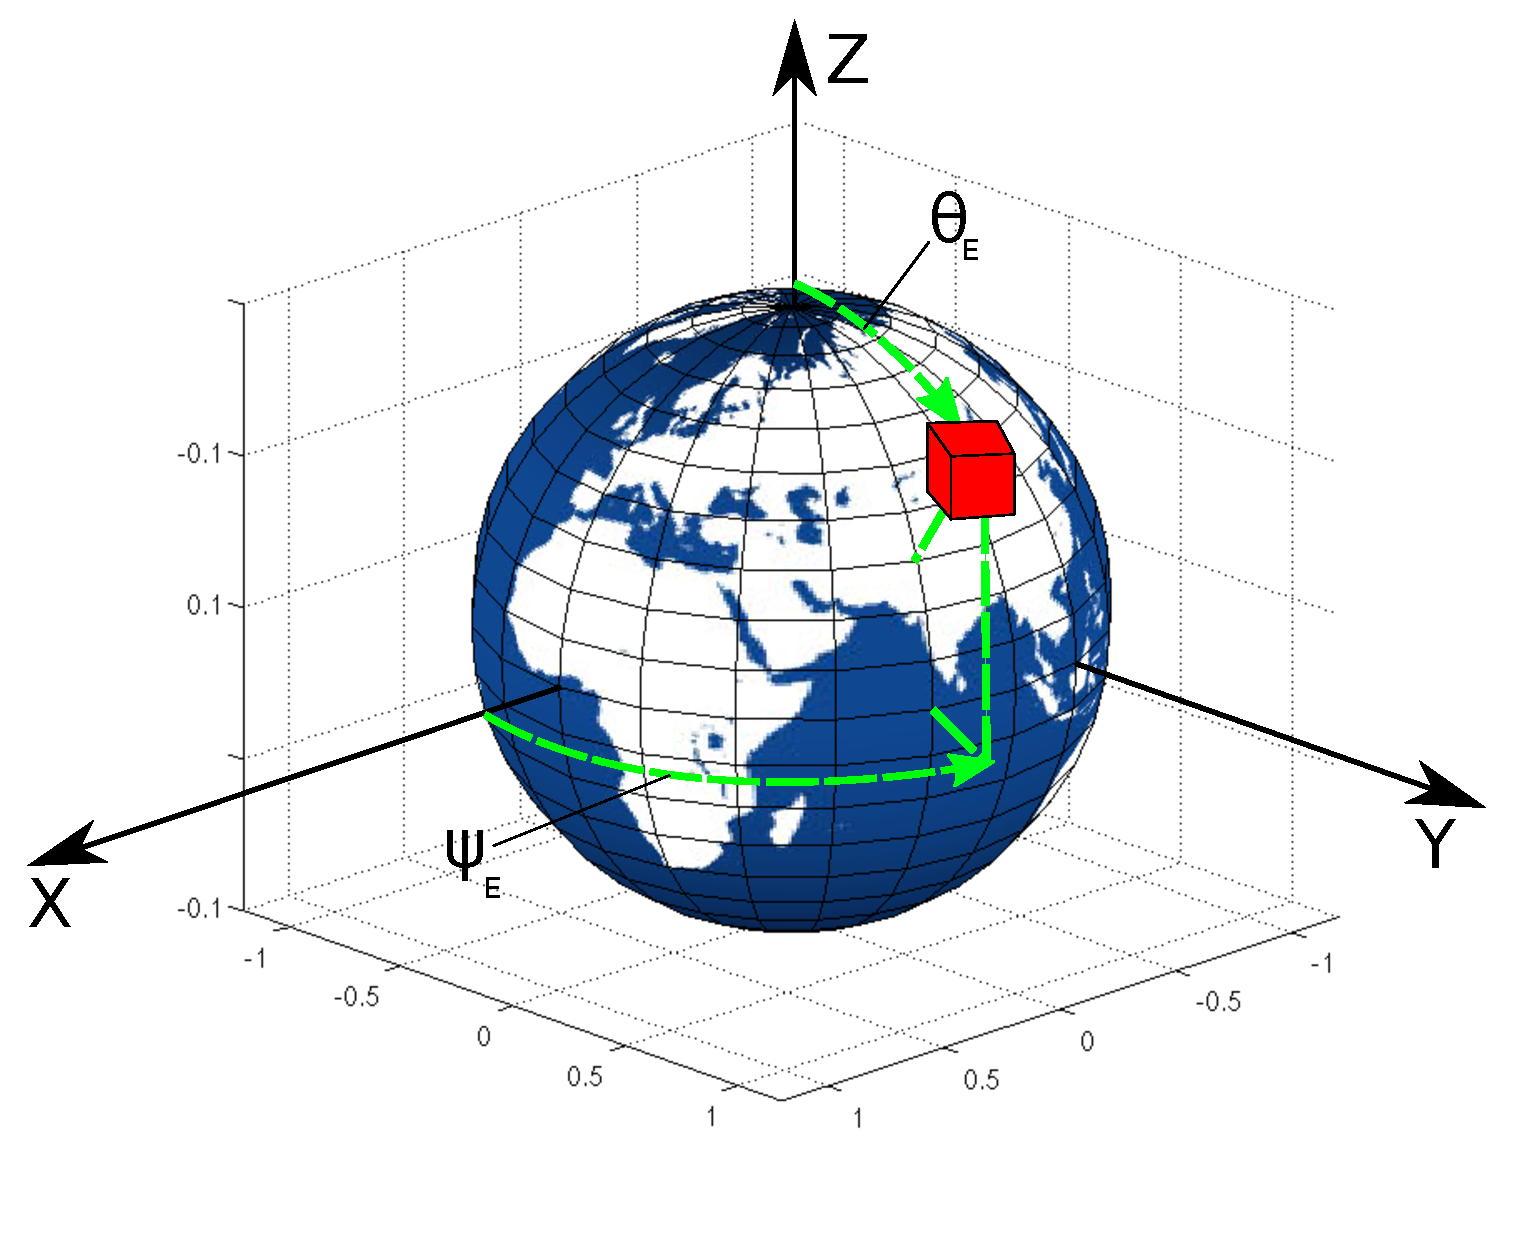
\includegraphics[height=100mm, width=120mm]{Figures/ECI.pdf}
  \end{center}
  \caption{Earth-Centered Inertial Frame and Spherical Coordinate Frame}\label{f:spherical}
\end{figure}
\noindent In order to connect these inertial coordinates ($x,y,z$) to
be used in the EMM2015 model, the latitude, longitude and height above
the surface of the Earth are required. To do this, the coordinates are
converted into spherical coordinates using the equations below.
\begin{equation}\label{e:spherical_coordinates}
  \begin{matrix}
    \rho = \sqrt{x^2+y^2+z^2} \\
    \phi_E = 0 \\
    \theta_E = cos^{-1}\left( \frac{z}{\rho}\right) \\
    \psi_E = tan^{-1}\left( \frac{y}{x}\right)
  \end{matrix}
\end{equation}
Note that $\rho,\phi_E,\theta_E,\psi_E$ are related to latitude and
longitude coordinates but not quite the same. In order to obtain the
latitude and longitude coordinates the following equations are
used. The height is simply the distance from the center of the ECI
frame minus the reference height from the approximation of Earth as an
ellipsoid ($R_{\Earth}=6,371,393~meters$). Note that the angles from Equation
\ref{e:spherical_coordinates} are converted to degrees. 
\begin{equation}
  \begin{matrix}
    \lambda_{LAT} = 90 - \theta_E\frac{180}{\pi}\\
    \lambda_{LON} = \psi_E\frac{180}{\pi} \\
    h = \rho - R_{\Earth}
  \end{matrix}
\end{equation}
The inputs are then the latitude, longitude and height. The output
from the EMM2015 model is in the East, North, Vertical (ENV) reference frame
where the x-axis is East pointing in the direction of the rotation on
the Earth, the y-axis is North pointing towards the North pole and
finally the z-axis is the Vertical component that is always pointing
radially away from the center of the Earth. In order to get the
coordinates into the ECI frame the coordinates must first me converted
to the North, East, Down reference frame (NED). In this case the
x-axis is pointing North, the y-axis pointing East and the z-axis is
always pointing towards the center of the Earth and called Down. The
equation to rotate from the ENV frame to NED frame is shown below.
\begin{equation}
  \begin{Bmatrix} \beta_x \\ \beta_y \\ \beta_z \end{Bmatrix}_{NED}
  = \begin{bmatrix} 0 & 1 & 0 \\ 1 & 0 & 0 \\ 0 & 0 & -1 \end{bmatrix} \begin{Bmatrix} \beta_x \\ \beta_y \\ \beta_z \end{Bmatrix}_{ENV}
\end{equation}
Once the magnetic field is in the NED reference frame it can then be
rotated to the inertial frame using the following equation where $\vec{\beta}_{NED}$ is the
magnetic field in the NED coordinate system and $\vec{\beta}_I$ is the
magnetic field in the inertial frame. 
\begin{equation}\label{e:sph_inertial}
  \vec{\beta}_I = {\bf T}_{IB}(0,\theta_E+\pi,\psi_E)\vec{\beta}_{NED}
\end{equation}
The matrix ${\bf T}_{IB}(\phi,\theta,\psi)$ represents the transformation
matrix from the spherical reference frame to the inertial reference
frame. Note that there is no rotation about the x-axis through
$\phi_E$ and the pitch rotation is augmented by $\pi$ because of the
switch between North, East, Down (NED) and the z-axis of the ECI
pointing through the North pole. The result of these equations, is the
ability to obtain the magnetic field  
across an entire orbit. Figure \ref{f:orbit} shows an example 56
degree inclination orbit, 600 km above the Earth's surface. The orbit
begins with the satellite above the equator and the prime meridian and
assumes the Earth does not rotate.
\begin{figure}[H]
  \begin{center}
  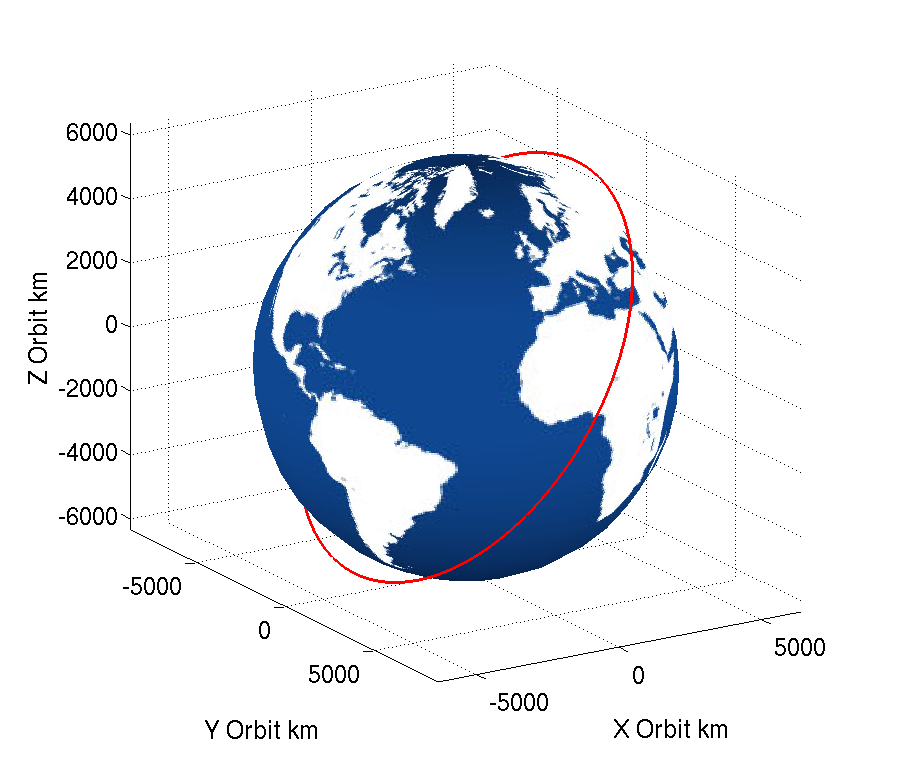
\includegraphics[height=70mm, width=80mm]{Figures/Earth_Orbit.png}
  \end{center}
  \caption{Example 56 Degree Inclination Orbit at 600 km above Earth's
  Surface}\label{f:orbit}
\end{figure}
Figure \ref{f:mag_orbit} shows the magnetic field during the orbit in the
inertial frame. PCI stands for Planet Centered Inertial which in this
case is the same as the ECI frame since the planet is Earth. 
\begin{figure}[H]
  \begin{center}
  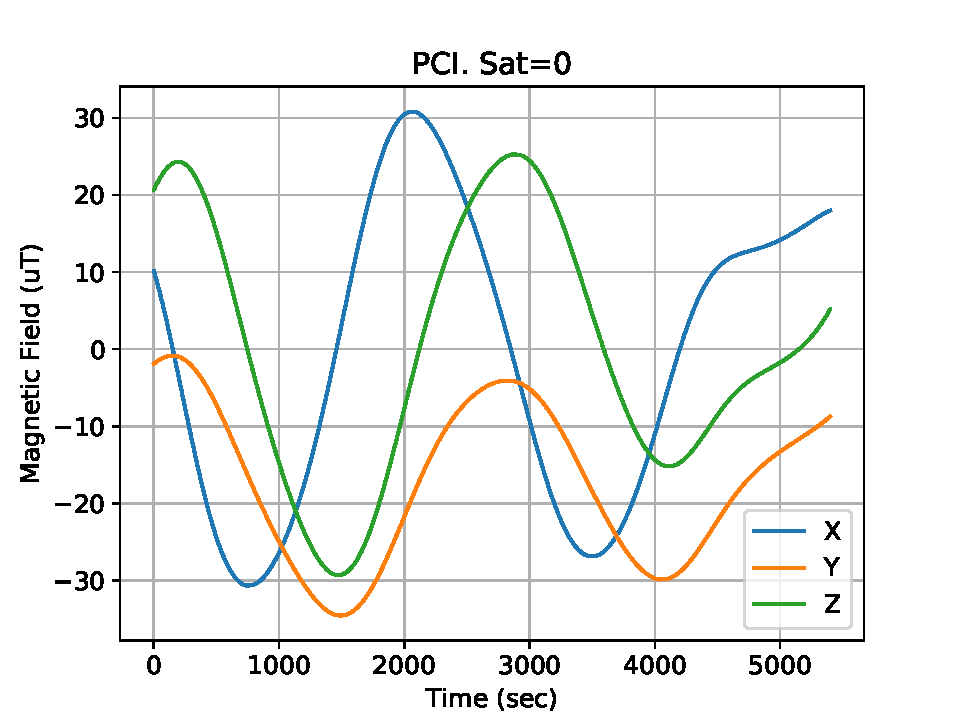
\includegraphics[width=90mm]{Figures/Magnetic_Field_Orbit}
  \end{center}
  \caption{Magnetic Field of Earth in Inertial Frame for 56 Degree
    Orbit at 600 km Above Surface}\label{f:mag_orbit}
\end{figure}

\subsection{Gravitational Models}

Two types of gravitational models can be used. The first is the
Newtonian gravitational model that assumes all planets are point
masses with no volume. The result of the gravitational field vector is
then
\begin{equation}
  F_{\Earth} = -G\frac{m_{\Earth} m_s}{r^2}\hat{r}
\end{equation}
where $G$ is the gravitational constant, $\Earth$ denotes the planet
applying the gravitational field, $m_\Earth$ is the mass of the
planet, $m_s$ is the mass of the satellite and $\vec{r}$ is a distance
vector from the center of the planet to the satellite. The vector
$\hat{r}$ is just the unit vector of $\vec{r}$ while $r$ is the
magnitude of $\vec{r}$.

The second gravitational field model stems from the
Earth Gravity Model (EGM2008) \cite{EGM2008} which can also be found
in the GeographicLib module \cite{GeographicLib}. This model compute's
Earths gravitational field at any point in three dimensional
space. The model takes in coordinates in the ECI frame and returns the
gravitational acceleration in the ECI frame thus no rotation is
required. Just like the EMM2015 model this model uses spherical
harmonics and a reference ellipsoid. The reference ellipsoid is then
updated with gravity disturbances such as non-uniform geoid
heights. This model is an upgrade from EGM84 and EGM96 which only
used models of order 180 and 360 respectively. The EGM2008 model as a
comparison uses a model of order 2190. Figure \ref{f:grav_orbit} shows
the gravitational acceleration vector during a 56 degree orbit at 600 km above the
Earth's surface. The x-axis has been non-dimensionalized to 
represent the entire orbit. Thus when the x-axis is equal to 100 the
satellite has completed one orbit.
\begin{figure}[H]
  \begin{center}
  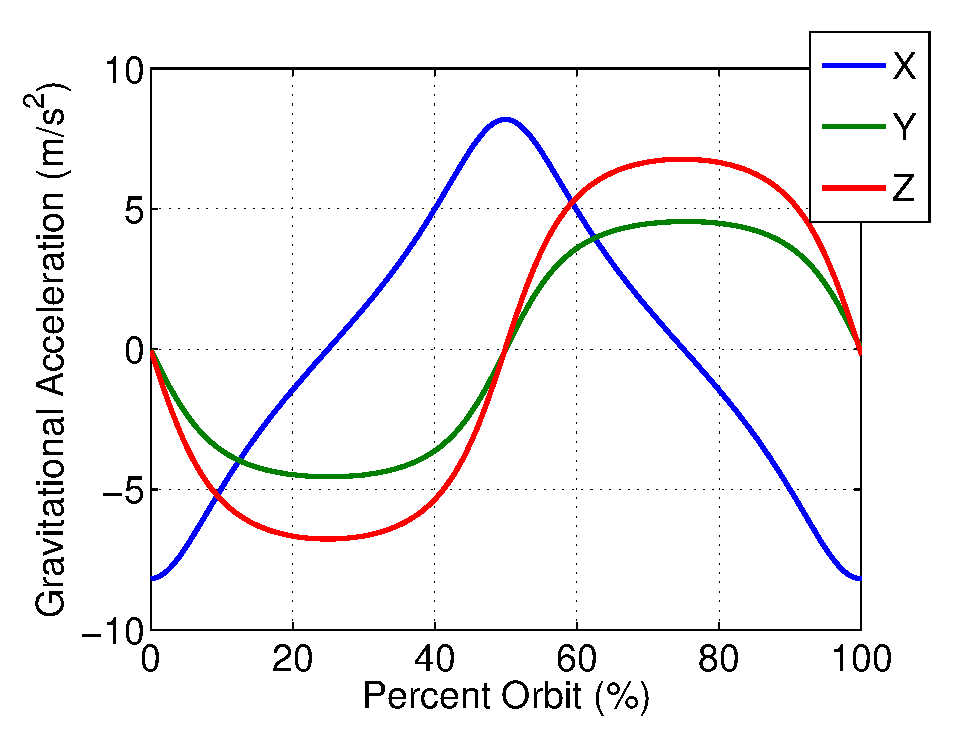
\includegraphics[height=80mm, width=100mm]{Figures/Gravity_Field_Orbit}
  \end{center}
  \caption{Gravitational Field of Earth in Inertial Frame for 56 Degree
    Orbit at 600 km Above Surface}\label{f:grav_orbit}
\end{figure}

\subsection{Earth Orbital Elements}\label{s:ephemeris}

Assuming that the Sun is the central inertial reference point, it is
possible to obtain the position of Earth at any point in time using
well documented orbital elements of the Earth. This formulation
follows the derivation by JPL and can be found at \cite{JPL}. In order
to obtain the position of the Earth, the Julian Day must be
obtained. The Julian Day of January 1st, 2019 is 2,458,485. The Julian
Day of January 1st, 2000 (which is the day of the last inertial frame
update) is 2,451,545. In order to obtain the Julian Day of the current
day, you simply need to count the number of calendar days from January
1st of 2000. Again I have listed the Julian day of January 1st, 2019
to help with this calculation. To compute the orbital elements of the
Earth you must then compute the number of centuries from January 1st,
2000 which is given by the equation below where J is the Julian day
and C is the number of centuries since 1/1/2000. 
\begin{equation}
  C = (J - 2,451,545)/36,525.0
\end{equation}
This number is then used in the equations below to obtain the current
semi-major axis, eccentricity, inclination, mean longitude, longitude
of perihelion and the longitude of the ascending node
respectively. The subscript $0$ denotes the orbital element in the
year 2000.
\begin{equation}
  \begin{matrix}
    a = (a_0 + \dot{a}C)AU \\
    e = e_0 + \dot{e}C \\
    i = i_0 + \dot{i}C \\
    L = L_0 + \dot{L}C \\
    \bar{w} = \bar{w}_0 + \dot{\bar{w}}C \\
    \Omega = \Omega_0 + \dot{\Omega}C
  \end{matrix}
\end{equation}
The parameters in the equation above for every planet can be found at
\cite{JPL}. Also, The term $AU$ is an astronomical unit which is equal
to 149,597,870,700 meters. For reference though the parameters for
Earth are shown below. Just in case you are reading this in the not so
distant future, these parameters are only valid until the year
2050. Also, the parameters below are for the Earth-Moon barycenter
which is the center of mass of the Earth and Moon.
\begin{table}
  \begin{center}
  \caption{Orbital Elements of Earth-Moon Barycenter}
\begin{tabular}{cccccc}
    a  &  e  & i & L & long.peri. ($\bar{w}$) & long.node. ($\Omega$)  \\
    \hline
    AU, AU/Cy &  rad, rad/Cy & deg, deg/Cy &  deg, deg/Cy & deg, deg/Cy &  deg, deg/Cy \\
    \hline 
    \hline 
    1.00000261 &  0.01671123  &  -0.00001531 &  100.46457166 &  102.93768193 &  0.0\\
    0.00000562 &  -0.00004392 &  -0.01294668 &   35999.37244981 &  0.32327364  &    0.0\\
    \hline
\end{tabular}
\end{center}
\end{table}
In the table, the first row is the value in the year 2000 and
the second row is the rate per century (Cy). Using these parameters,
compute the argument of the perihelion $w = \bar{w} - \Omega$ and the
mean anomaly $M = L - \bar{w}$. Note that for planets Jupiter, Saturn,
Uranus and Neptune, the mean anomaly has a different form. Basically
anything past the asteroid belt. With the mean anomaly compute you
must modulus this value such that M is between plus or minus 180
degrees. Once that's done you must solve for the eccentric anomaly (E)
using the Kepler equation below where $e^*$ is the eccentricity in
degrees $e^* = 180e/\pi$. 
\begin{equation}
  M = E-e^*sin(E)
\end{equation}
Solving this numerically is pretty simple and only requires a few
iterations of the loop below using the C++ programming language. This
loop can easily be adapted to any language on modern computers. C++ is
shown here in the event this is used for embedded processors in future
satellite systems. 
\begin{verbatim}
  E = M + e*180.0/PI*sin(M*PI/180.0);
  dM = 1;
  dE = 0;
  while (abs(dM) > 1e-6) {
    dM = M - (E - e*180.0/PI*sin(E*PI/180.0));
    dE = dM/(1.0-e*cos(E*PI/180.0));
    E += dE;
  }        
\end{verbatim}
At this point the spatial coordinates can be obtained in the planet's
orbital plane where the semi-latus rectum or sometimes simply called
the parameter is $p=a(1-e)$. 
\begin{equation}
  \begin{Bmatrix} x' \\ y' \\ z' \end{Bmatrix} = \begin{Bmatrix} a(cos(\pi E/180) - e)
    \\ a\sqrt{1-e^2}sin(\pi E/180) \\ 0 \end{Bmatrix}
\end{equation}
Notice that the value $z'$ is zero. This is because orbits are all two
dimensional. In order to obtain the coordinates of the planet in the
J2000 ecliptic plane, the equation below is used which is similar to
the standard Euler angle transformation matrix only the 3-1-3 rotation
sequence is used rather than 3-2-1. 
\begin{equation}
  \begin{Bmatrix} x \\ y \\ z \end{Bmatrix}_{J2000} = \begin{bmatrix} c_wc_{\Omega}-s_ws_{\Omega}c_i &
    -s_wc_{\Omega}-c_ws_{\Omega}c_i & 0
    \\ c_ws_{\Omega}+s_wc_{\Omega}c_i &
    -s_ws_{\Omega}+c_wc_{\Omega}c_i & 0 \\
    s_ws_i & c_ws_i & 0 \end{bmatrix} \begin{Bmatrix} x' \\ y' \\ z' \end{Bmatrix}
\end{equation}
Running through this formulation for all the planets in the Solar
System including Pluto it is possible to plot the position of all
planets. The figures below are for January 1st, 2019.
\begin{figure}[H]
  \begin{center}
  \begin{tabular}{cc}
  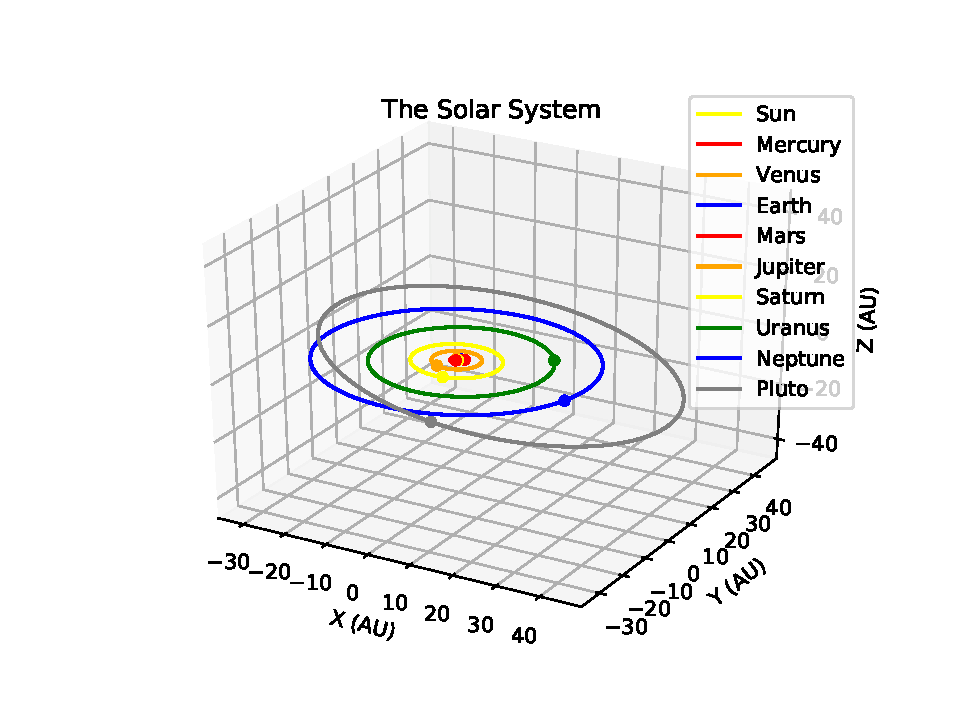
\includegraphics[height=70mm, width=80mm]{Figures/all_planets_isometric.pdf}&
  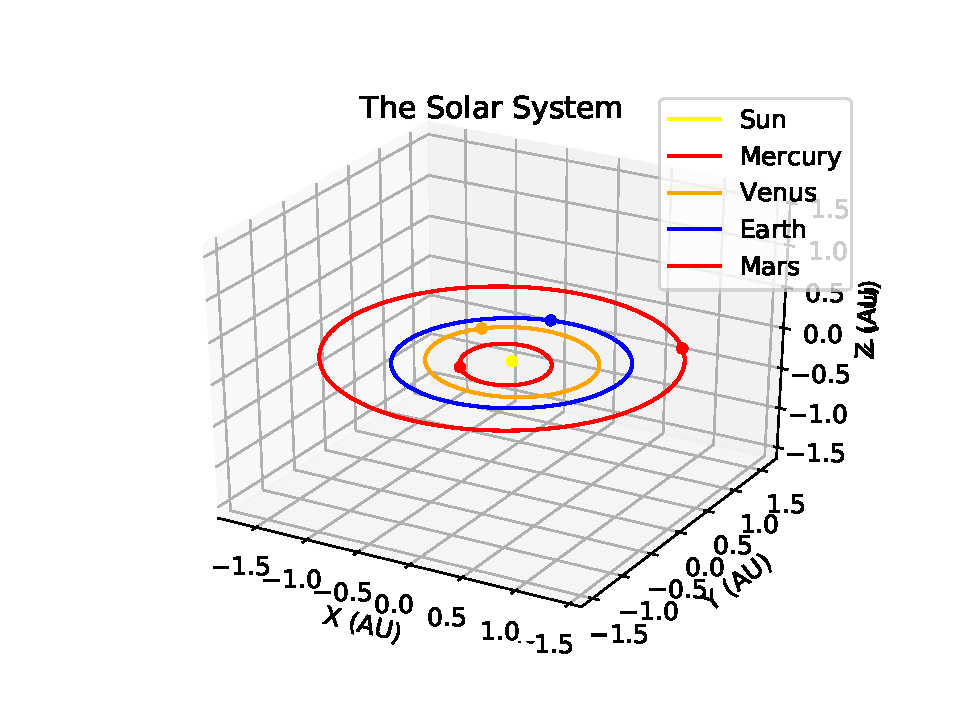
\includegraphics[height=70mm, width=80mm]{Figures/inner_planets_isometric.pdf}\\
  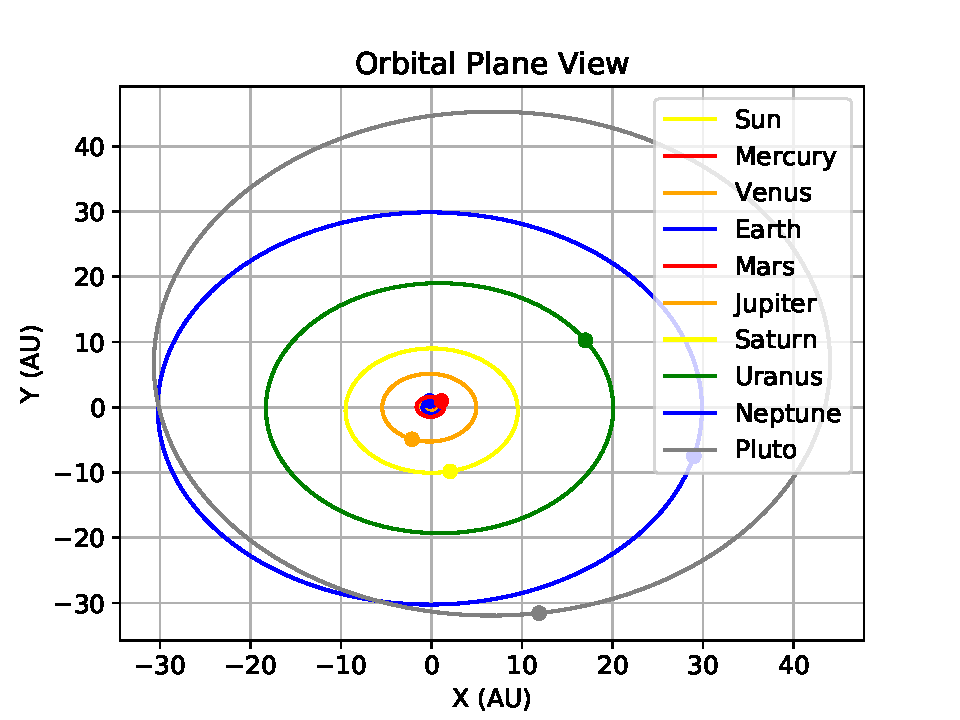
\includegraphics[height=70mm, width=80mm]{Figures/top_down_view_all_planets.pdf}&
  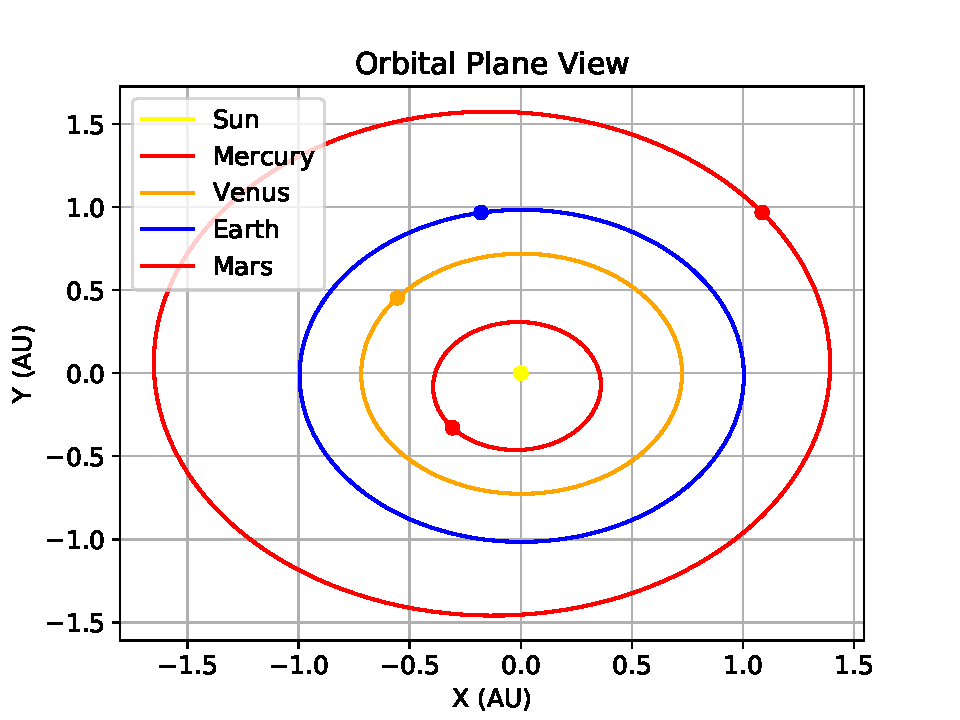
\includegraphics[height=70mm, width=80mm]{Figures/inner_planets_top_down.pdf}\\
  \end{tabular}
  \end{center}
  \caption{Position of Planets using Orbital Elements}
\end{figure}

\section{External Forces and Moments}

In addition to gravity acting on the satellite, other forces also act
on the satellite. For a 1U CubeSat, the gravity gradient over 10 cm is about
$0.24~\mu m/s^2$ using the EGM2008 model. Multiplying this 
acceleration by a $1~kg$ mass and applying a $10~cm$ moment arm yields
a moment of about $2.4 \times 10^{-8}~N-m$. Aerodynamic torques could
be as large as $1.5 \times 10^{-10}~N-m$ assuming the aerodynamic
center is 5~cm away from the center of mass. Typical magnetorquers operate
in the vicinity of $3.0 \times 10^{-6}~N-m$, assuming a current of $0.04~A$, an area of
$0.02~m^2$, 84 turns and a magnetic field of $40,000~nT$. Using
these calculations, magnetorquers are two orders of magnitude
larger than gravity torques and four orders of magnitude larger than
aerodynamic torques. It is important to keep these values in mind when
neglecting certain parameters \cite{Radiation,AndersonD,Density_Model}.

\subsection{Propulsion Model}

Each satellite is equipped with $N_P$ thrusters that have a fixed
$I_{sp}$. The mass flow rate of each thruster is given by the equation
below where $p$ is the force of the thruster.
\begin{equation}
  \dot{m}_i = \sigma_i\frac{p}{9.81~I_{sp}}
\end{equation}
Each thruster is either on or off as given by the variable $\sigma$
which is either a 1 or a 0. When the thruster is on, the force
applied is equal to $p$ and when the thruster is off the thrust
applied is equal to zero. Thus in this fashion to total mass flow rate
per unit time of the entire satellite is just a sum of all the pulses.
\begin{equation}
  \dot{m} = \frac{p}{9.81~I_{sp}}\sum\limits_{i=1}^{N_P}\sigma_i
\end{equation}
It is assumed that the time response of the
thrusters is instantaneous during power up and power down. There is a
delay between pulses and the thrusters only stay on for a fixed time
thus the thrusters are pulsed in a square wave fashion with a certain
duty cycle. The force applied is simply equal to the force times a
unit vector that is aligned with the axis of the thruster. The total
force applied to each satellite is then given by the formula below.
\begin{equation}
  \vec{F}_P = p\sum\limits_{i=1}^{N_P}\sigma_i\hat{n}_{Pi}
\end{equation}
The total moment applied to the satellite is simply the force applied
crossed with a vector from the center of mass of the satellite to the
center of mass of the thruster.
\begin{equation}\label{e:propulsion}
  \vec{M}_P = p\sum\limits_{i=1}^{N_P}\sigma_i{\bf S}(\vec{r}_{Pi})\hat{n}_{Pi}
\end{equation}

\subsection{Magnetorquer Model}

The magnetorquer model assumes that three magnetorquers are aligned in
such a way that the magnetic moment produced by each magnetorquer is
aligned with the principal axes of the body frame of the
satellite. Each magnetorquer is controlled independently such that
$\vec{i}_M = [i_x,i_y,i_z]^T$ which is the applied current in each
magnetorquer. The magnetic moment is then given by the equation below 
\begin{equation}\label{e:magmoment}
  \vec{\mu}_M = nA\vec{i}_M
\end{equation}
where $n$ is the number of turns in the coil 
of each magnetorquer and $A$ is the area of the magnetorquer. For
simplicity it is assumed that all magnetorquers have the same area and
same number of turns. The torque produced by all magnetorquers is then
simply found by crossing the magnetic moment with the magnetic field
of the Earth in the Body reference frame.
\begin{equation}\label{e:magtorque}
  \vec{M}_M = {\bf S}(\vec{\mu}_M){\bf T_{BI}}(\vec{q})\vec{\beta}_I
\end{equation}
In order to obtain the magnetic field vector in the body frame, the
inertial magnetic field vector must be rotated into the body frame of
the satellite. In component form, equation (\ref{e:magtorque}) reduces to the following
equation using the identity that $\vec{a}\times\vec{b}=-\vec{b}\times\vec{a}$
\begin{equation}\label{e:magtorquecomponent}
  \begin{Bmatrix} L_M \\ M_M \\ N_M \end{Bmatrix} = nA\begin{bmatrix} 0 & \beta_z & -\beta_y \\ -\beta_z & 0 &
  \beta_x \\ \beta_y & -\beta_x & 0 \end{bmatrix}\begin{Bmatrix} i_{x}
    \\ i_{y} \\ i_{z} \end{Bmatrix}
\end{equation}
where $\beta_x,\beta_y,~\beta_z$ are the components of the magnetic
field in the body frame of the satellite. The moments $L,M,N$ are thus
the control torques that rotate the satellite as seen in equation
(\ref{e:pqrdot}). 

\section{Control Schemes}

Many control schemes are needed to orient a satellite and all depend
on the application. In LEO magnetorquers can be used to detumble a
satellite while thrusters must be used in deep space. In addition
reaction wheels can be used to detumble a satellite anywhere in space
provided the angular momentum in the satellite does not saturate the
reaction wheels. Sections that follow detail the control schemes
typically utilized on small sats. 

\subsection{B-dot Controller}

In LEO, the standard B-dot controller reported in many sources
(\cite{Leomanni2012},\cite{Lovera2015},\cite{WInstitute},\cite{SanyalDick})
can be used to de-tumble a satellite. The standard B-dot controller
requires the magnetorquers to follow the control law shown below
\begin{equation}\label{e:bdotcompact}
  \vec{\mu}_B = k{\bf S}(\vec{\omega}_{B/I}){\bf T}_{BI}(\vec{q})\vec{\beta}_I
\end{equation}
where $k$ is the control gain. Using equation (\ref{e:magmoment}) it
is possible to write the current in component form again
using the identity that $\vec{a}\times\vec{b}=-\vec{b}\times\vec{a}$
\begin{equation}\label{e:bdot}
  \begin{Bmatrix} i_{x}
    \\ i_{y} \\ i_{z} \end{Bmatrix} = \frac{k}{nA}\begin{bmatrix} 0 & \beta_z & -\beta_y \\ -\beta_z & 0 &
  \beta_x \\ \beta_y & -\beta_x & 0 \end{bmatrix}\begin{Bmatrix} p
    \\ q \\ r \end{Bmatrix}
\end{equation}
This equation can then be substituted into equation
(\ref{e:magtorquecomponent}) to produce the total torque on the
satellite assuming that the magnetorquers can provide the necessary
current commanded by equation (\ref{e:bdot}).
\begin{equation}\label{e:bdotfinal}
  \begin{Bmatrix} L \\ M \\ N \end{Bmatrix} = -k \begin{bmatrix}
    \beta_y^2 + \beta_z^2 & -\beta_x\beta_y & -\beta_x\beta_z
    \\ -\beta_x\beta_y & \beta_x^2 + \beta_z^2 & -\beta_y\beta_z \\
    -\beta_x\beta_z & -\beta_y\beta_z & \beta_x^2 +
    \beta_y^2 \end{bmatrix} \begin{Bmatrix} p
    \\ q \\ r \end{Bmatrix} 
\end{equation}
The goal of the controller here is to drive
$\vec{\omega}_{B/I}\rightarrow 0$. The literature will show that
this is not completely achieved \cite{Celani}. There are multiple
explanations for this. For starters, equation (\ref{e:magtorque})
assumes that the magnetic moment is not co-linear with the magnetic
field of the Earth. If it is, the result is zero torque applied to the
satellite. Furthermore, equation (\ref{e:bdot})
results in zero current if the angular velocity vector of the
satellite is co-linear with the magnetic field. Thus, if the magnetic
field vector, angular velocity vector or the magnetic moment vector
are co-linear, the torque applied to the satellite will be zero. If a
new operator is defined such that
\begin{equation}
  {\bf W}({\bf T}_{BI}(\vec{q})\vec{\beta}_I) = \begin{bmatrix}
    \beta_y^2 + \beta_z^2 & -\beta_x\beta_y & -\beta_x\beta_z
    \\ -\beta_x\beta_y & \beta_x^2 + \beta_z^2 & -\beta_y\beta_z \\
    -\beta_x\beta_z & -\beta_y\beta_z & \beta_x^2 +
    \beta_y^2 \end{bmatrix}
\end{equation}
it is easy to see that the torque applied to a satellite is then
simply the angular velocity vector multiplied by this transition
matrix. If this transition matrix is put into row-reduced-echelon form
it is easy to see that the determinant of this matrix is equal to
zero (\cite{carlen2006linear}).
\begin{equation}
  rref({\bf W}({\bf T}_{BI}(\vec{q})\vec{\beta}_I) = \begin{bmatrix} 1 & 0
    & -\beta_x/ \beta_z \\ 0 & 1 & -\beta_y/ \beta_z \\ 0 & 0 & 0 \end{bmatrix}
\end{equation}
A zero determinant means that there exists a vector
$\vec{\omega}_{B/I}$ that will result in zero torque for a given value
of the magnetic field. This is typically avoided since the
magnetic field of the Earth is time and spatially varying
which results in a transition matrix that changes over time due to
orientation changes in the satellite as well as changes in the satellite's
orbit. However, for low inclination orbits, it's possible for the
magnetic field to stay relatively constant with $\beta_x \approx
\beta_y \approx 0$. If the satellite is tumbling about the yaw axis such
that $p=q=0$, the yaw torque on the satellite ($N$) will be
zero. Using this simple controller, there is no way to
remove the remaining angular velocity from the satellite unless
reaction wheels are used.

\subsection{Reaction Wheels}

Assuming each reaction is aligned with a principal axis of inertia the
control scheme is extremely simple. When the wheels are not aligned
the derivation will proceed similar to the reaction control thruster
section. The derivation here will just be for the aligned case. In
this analysis it is assumed that a torque can be applied to the
reaction wheel and thus the angular velocity of the reaction wheel
$\alpha_{Ri}$ can be directly controlled. Assuming this a simple PD
control law can be used to orient the satellite at any desired
orientation using Euler angles for this control law since the
satellites are aligned with the principal axes of rotation \cite{etkins}.
\begin{equation}
  \alpha_{Ri} = -k_p(\epsilon_i-\epsilon_{desired})-k_d(\omega_i-\omega_{desired})
\end{equation}
In the equation above $\epsilon$ denotes either roll $\phi$, pitch
$\theta$ or yaw $\psi$ depending on which reaction wheel is being
used. The Euler angles in this case would be obtained by converting
the quaternions to Euler angles as defined in Section \ref{s:quat}.
In order to design and select reaction wheels the maximum angular
momentum of the satellite must be obtained by assuming the worst case angular
velocity times the moment of inertia of the satellite.
\begin{equation}
  H_{required} = n||I_s\vec{\omega}_{MAX}||
\end{equation}
With this reaction wheels can be selected based on this worst case
scenario plus a safety factor of $n$ which is typcially set to 2 in
spacecraft operations. If reaction wheels cannot be used in the event
of saturation or other issues reaction control thrusters can be
used. Typically a value of $|\vec{\omega}_{MAX}|=5^o/sec$ is used. 

\subsection{Reaction Control Thrusters}

The control law for the thrusters is a bit complex if the location of
thrusters is not know apriori. If the location {\it is} known then
simple PID control laws can be generated by applying pure couples to
the correct thrusters that activate the correct axes. If the location
{\it is not} known then the following derivation will suffice. There
are $N_P$ thrusters and only 3 degrees of freedom that need to be
controlled; thus, the system is an overactuated system. Using equation
\ref{e:propulsion}, the equation can be written in matrix form as
given by the equation below where $\vec{M}_p$ is replaced by
$\vec{M}_{desired}$. The equation for $\vec{M}_{desired}$ is generated
using a similar PD control law as the reaction wheels. 
\begin{equation}
  \vec{M}_{desired} = p[{\bf S}(\vec{r}_{P1})\hat{n}_{P1}~~{\bf
      S}(\vec{r}_{P2})\hat{n}_{P2}~~\hdots~~{\bf
      S}(\vec{r}_{P{N_p}})\hat{n}_{P{N_p}}]\vec{\sigma} = {\bf M}\vec{\sigma}
\end{equation}
Since ${\bf M}$ is a $3\times{N_P}$ matrix its impossible to simply
invert the matrix and solve for the vector of pulses
$\vec{\sigma}$. Instead, Lagrange's method was used to find the vector
of pulses \cite{lagrange}.
\begin{equation}
  \vec{\sigma} = {\bf M}^T\left({\bf M}{\bf M}^T\right)^{-1}\vec{M}_{desired}
\end{equation}
Note that a similar equation can be derived for
$\vec{F}_{desired}$. The solution to the equation above results in
values of $\sigma$ that are bigger than 1 and sometimes negative. If a
value in this vector is bigger than 0 the value is set to 1 and
if the value is negative the value is set to 0. Thus, the solution
does not yield an exact solution but it does allow for flexibility in
the number of thrusters and their respective orientations. Sizing of
the thrusters depends on many independent variables 
including the thrust $T$ and the $I_{sp}$. Using the $I_{sp}$ the exit
velocity of the thruster can be obtained by using the equation below
\begin{equation}
  v_e = I_{sp}g_0
\end{equation}
where $g_0$ is the gravitational acceleration of the Earth at
sea-level. Then the mass flow rate of the thruster can be obtained
using the equation below.
\begin{equation}
  \dot{m}_P = T/v_e
\end{equation}
Using this mass flow rate total propellant mass required can be
computed assuming a certain duty cycle.

\subsection{Cross Products of Inertia}

An interesting form of control is to take advantage of momentum
dumping. Looking at the equation for angular acceleration again (Eqn \ref{e:pqrdot}) this
equation can be simplified for certain cases. For example, if the roll
rate of the satellite is set to be non-zero while the pitch rate and
yaw rates are set to zero it is easy to see that if the inertia is
diagonal the derivative of angular velocity is zero. However, if the
cross products of inertia are given by the matrix below
\begin{equation}
  {\bf I}_s = \begin{bmatrix} I_{xx} & I_{xy} & I_{xz} \\ I_{xy} &
    I_{yy} & I_{yz} \\ I_{xz} & I_{yz} & I_{zz} \end{bmatrix}
\end{equation}
the derivative of angular velocity becomes
\begin{equation}
  \dot{\vec{\omega}}_{B/I} = I_S^{-1} \left (\begin{Bmatrix} 0
    \\ -I_{xz}p^2 \\ I_{xy}p^2 \end{Bmatrix} \right )
\end{equation}
again assuming the roll rate is non zero and the pitch rate is
zero. This result shows that momentum can be transferred to different
axes provided the cross products of inertia are non-zero. 

\section{Numerical Integration Techniques}

\subsection{Linear Dynamics}

The nonlinear dynamics formulated above can be placed into standard
nonlinear affine form as shown below after much simplification of
terms
\begin{equation}
  \dot{\vec{x}} = \vec{f}(\vec{x}) + \vec{g}(\vec{x})\vec{u}
\end{equation}
where $\vec{u}$ is the control input which could be the forces and
moments from reaction wheels or thrusters. The equation above can be
linearized to give the equation below. 
\begin{equation}
  \Delta \dot{\vec{x}} = {\bf A}\Delta {\vec{x}} + {\bf B}\Delta \vec{u}
\end{equation}
where $\Delta \vec{x} = \vec{x} - \vec{x}_e$ and $\vec{x}_e$ is an
equilibrium point. In this formulation ${\bf A} = \partial \vec{f}/\partial \vec{x}$. and 
${\bf B} = \partial \vec{g}/\partial \vec{x}$

\subsection{Euler's Method}

The equations of motion above can be integrated using Euler's method
which is a crude first order method to approximate the time series
solution \cite{Chapra_MEANALYSIS}. Note that this method is prone to a 
significant amount of instability unless the timestep is very small. 
\begin{equation}
  \begin{matrix}
    \vec{x}_{k+1} = \vec{x}_k + \dot{\vec{x}}(t_k,\vec{x}_k) \Delta t \\
    \dot{\vec{x}}(t_k,\vec{x}_k) = \vec{f}(\vec{x}_k) + \vec{g}(\vec{x}_k)\vec{u}_k
  \end{matrix}
\end{equation}

\subsection{Runge-Kutta-4}

The RK4 algorithm is the standard in numerical integration and is
given in the equation below \cite{Chapra_MEANALYSIS}. The derivative
of the quaternions is the same in RK4 as it is in Euler's method. This
method is superior to RK4 in that it will converge faster as a
function of timestep.
\begin{equation}
  \begin{matrix}
    \vec{k}_1 = \dot{\vec{x}}(t_k,\vec{x}_k)\\
    \vec{k}_2 = \dot{\vec{x}}(t_k+\Delta t/2,\vec{x}_k+\vec{k}_1\Delta t/2)\\
    \vec{k}_3 = \dot{\vec{x}}(t_k+\Delta t/2,\vec{x}_k+\vec{k}_2\Delta t/2)\\
    \vec{k}_4 = \dot{\vec{x}}(t_k+\Delta t,\vec{x}_k+\vec{k}_3\Delta t)\\
    \vec{k} = \frac{1}{6}(\vec{k}_1 + 2\vec{k}_2 + 2\vec{k}_3 + \vec{k}_4)\\
    \vec{x}_{k+1} = \vec{x}_k + \vec{k} \Delta t \\
  \end{matrix}
\end{equation}

\subsection{Discrete Dynamics}

It is often useful for modern computers to write the equations of
motion in discrete form....

\section{Attitude Determination}

Attitude determination is a fundamental portion of the ADACS board and
requires the vehicle to determine it's orientation with respect to an
inertial frame. The sections that follow detail the sensors and
fundamental attitude determination algorithms derived thus far. 

\subsection{Sensor Overview}

There are a multitude of sensors that are typically used on board
small sats. Note that most satellites use a combination of these
sensors rather than using all of them on one single satellite.

\begin{enumerate}[itemsep=-5pt]
  \item {\bf Magnetometers:} Only used in LEO, they measure the
    magnetic field in the body frame $\vec{\beta}_B = [\beta_x,\beta_y,\beta_z]^T$.
    \item {\bf Rate Gyros:} These sensors measure the angular velocity
      of the spacecraft in the body frame $p,q,r$.
    \item {\bf Solar Sensors:} These sensors can be coarse analog
      sensors with an accuracy of 45 degrees or can be high precision
      digital sensors that have accuracy down to 1 degree. Sun senors
      return an azimuth $\upsilon$ and declination $\delta$ angle which can be then
      translated into a vector in the body frame $\vec{S}_B$.
    \item {\bf Horizon Sensors:} Horizon sensors are typically used in
      LEO as they find the horizon of the Earth and use that for
      orientation information. These sensors also return an azimuth
      and declination angle that can be translated into a body frame
      vector $\vec{H}_B$.
      \item {\bf Startrackers:} Startrackers utilize a large aperture
        digital camera to photograph a starmap within the field of
        view of the lens. The photographed stars are then cross
        referenced with a starmap database and return the full
        quaternion vector.
\end{enumerate}

Some issues arise with all of these sensors. For example,
magnetometers must be activated when magnetorquers are turned off
otherwise those artificial magnetic fields will pollute the data. Rate
gyros are prone to drift while solar sensors can be quite
inaccurate. Startrackers also run the risk of being blinded by the Sun
and/or the Moon thus it is possible to design an
attitude determination algorithm that utilizes the Sun's ephemeris data
along with the Moon's ephemeris data in the event that the startracker
is obscured by the Sun/Moon.

\subsection{Low Earth Orbit}

In LEO the main algorithm begins with obtaining the magnetic field in
the body frame using magnetometers $\vec{\beta}_B$. A Sun measurement is
then taken using a Sun sensor $\vec{S}_B$. Once those two independent
body frame measurements are taken the inertial reference vectors must
be obtained from a database. Startrackers have this database built in;
however, for the magnetic field and the Sun vector these must be
obtained from a separate database as discussed in Section
\ref{s:ephemeris}. The idea is that if the position of the Earth is
known then the position of the Sun with respect to the Earth is also
known. The magnetic field vector can be 
obtained from the IGRF model as discussed in Section
\ref{s:magnetic_field}. The magnetic field vector in the inertial
frame is given as $\vec{\beta}_I$. Note that the IGRF model requires
the latitude and longitude to be known. Thus, in LEO a GPS is required
to feed into the database. The inertial Sun vector $\vec{S}_I$ only
requires the Julian time which can be obtained from GPS as well. The julian time is
based on the julian day as explained in Section \ref{s:ephemeris}. 

\subsection{Deep Space}

As explained earlier, in deep space it is possible to obtain a vector
to the Moon to be used in the attitude determination algorithm. The
Moon sensor would give a vector to the Moon in the body frame
$\vec{M}_B$ while an inertial vector would be needed $\vec{M}_I$. This
inertial Moon vector could be obtained via the Moon's
ephemeris data which could be loaded onto the satellite's processor
and use the orbital elements of the Moon to determine its position
relative to the Earth. However, the Moon's ephemeris data would more
than likely give the Moon's position relative to the Earth
($\vec{r}_{\Earth \rightarrow \Moon}$). The vector $\vec{M}_I$ would
then be given by
\begin{equation}
  \vec{M}_I = \vec{r}_{\Earth \rightarrow \Moon} - \vec{r}_{B}
\end{equation}
where $\vec{r}_B$ is the satellite's position relative to the
Earth. Note however that the position of the satellite relative to the
Earth would need to be obtained via the Deep Space Network (DSN) and a
combination of state estimation by integrating the orbital
equations. The reference paper \cite{Munoz} is a great paper that
details all the different kinds of sensors and their algorithms. This
section will eventually be supplemented by the material in that
reference paper.

\subsection{Algorithm}

The initial attitude determination algorithm itself requires two
independent vectors. As stated previously, startrackers provided a
large enough aperture and enough stars to produce the full
quaternion by obtaining multiple unique vectors to unique
stars. Multiple solar sensors or multiple magnetometers unfortunately
do not obtain non-unique vectors and the algorithm fails. In LEO this
is typically done with solar sensors and magnetometers but it can be
done with star trackers. In deep space it is typically done with
startrackers but it could be possible to obtain a Moon vector that
would require a Moon sensor.

The derivation below is done for the LEO case with a Sun and magnetic
field measurement. The derivation is identical for the deep space case
with a Moon sensor simply by substituting the magnetic field
measurment with a Moon measurement. Every vector is first normalized to obtain
$\hat{\beta}_B,\hat{\beta}_I,\hat{S}_B,\hat{S}_I$. A triad is then created
from body frame vectors using the equations below.
\begin{equation}
  \begin{matrix} \hat{f}_1 = \hat{S}_B & \hat{f}_2 = \hat{f}_1 \times
    \hat{\beta}_B & \hat{f}_3 = \hat{f}_1 \times \hat{f}_2 \end{matrix}
\end{equation}
The matrix ${\bf F}$ is then created using the triad as an orthonormal basis
$F = [\hat{f}_1,\hat{f}_2,\hat{f}_3]$. Similar equations are used for
the inertial measurements. 
\begin{equation}
  \begin{matrix} \hat{g}_1 = \hat{S}_I & \hat{g}_2 = \hat{g}_1 \times
    \hat{\beta}_I & \hat{g}_3 = \hat{g}_1 \times \hat{g}_2 \end{matrix}
\end{equation}
The matrix ${\bf G}$ is then created just as the ${\bf F}$ matrix such
that ${\bf G} =
[\hat{g}_1,\hat{g}_2,\hat{g}_3]$. The transformation from inertial to
body frame is then created using the formula below.
\begin{equation}
  {\bf T}_{BI} = {\bf FG}^T
\end{equation}
This matrix above is similar to the matrix in equation \ref{e:TIB} and
thus the Euler angles can be extracted from the matrix itself using
the formulation defined in Section \ref{s:Euler_Angles}. Euler can
then be converted to quaternions if needed. Note that it is relatively
easy to extract Euler angles from the ${\bf T}_{IB}$ matrix, it is not so
simple to extract quaternions. This is due to the fact that for every
orientation there exists two quaternions that represent this
space. Thus, it is more ideal to obtain Euler angles from the
transformation matrix and then convert them to quaternions.

\section{State Estimation}

\subsection{Sensor Measurement} \label{s:measurements}

During the standard estimation procedure, it is assumed that
measurements are made that relate to the state or the state is
directly measured. If the state is directly measured like star trackers no special formulation need to
made. However, other sensors such as Sun sensors, magnetometers and
horizon sensors measure a vector in 3-D space. In general a
measurement $\bar{y}_k$ can be expressed by the nonlinear equation
shown below where $\vec{x}$ is the state vector. 
\begin{equation}
  \bar{y}_k = \vec{h}(\vec{x}_k) + \vec{\nu}_k
\end{equation}
The vector $\vec{\nu}_k$ is noise associated with the sensor
\cite{Munoz,cassidis}. If the system is linearized about some
equilibrium point the measurement equation can be written as
\begin{equation}
  \bar{y}_k = {\bf h}_k\vec{x}_k + \vec{\nu}_k
\end{equation}
where ${\bf h}_k = \partial \vec{h}/\partial \vec{x}$. 
It's easy to see here that in the case of the star tracker the matrix
${\bf h}_k$ is just the identity matrix. The noise vector
$\vec{\nu}_k$ is assumed to be gaussian white noise while the
covariance $cov()$ is given by the equation below using the
expectation operator ${\bf E}()$.
\begin{equation}
  cov(\vec{\nu}_k) = {\bf E}(\vec{\nu}_k\vec{\nu}_k^T) = {\bf R}_k
\end{equation}
If a measurement is made by a
Sun sensor or similar where a vector in 3-D space can be compared to a
known inertial reference vector the measurement update can be given as 
\begin{equation}
  {\bar{r}^B}_k = {\bf T}_{BI}(\vec{q}_k){\vec{r}^I}_k + \vec{\nu}_k
\end{equation}
where ${\bar{r}^B}_k$ is a measurement in the body reference frame at
time $t_k$. The angular velocity measurement in particular can be denoted as
$\bar{\omega}_k$. Measurements are typically polluted with bias and
white noise. For example, the angular velocity measurement can be
given as
\begin{equation}
  \bar{\omega} = \vec{\omega} + \vec{b} + \vec{\eta}_g
\end{equation}
where $\vec{b}$ is a bias that has dynamics given by
$\dot{\vec{b}}=\vec{\eta}_b$. The vectors $\vec{\eta}_g$ and
$\vec{\eta}_b$ are standard Gaussian white noise vectors. Typically
white noise can be filtered out using lowpass filters, complimentary
filters or even Kalman Filters while bias can just be
substracted. Thus, the estimate for the angular velocity can be
written as
\begin{equation}
  \tilde{\omega} = \bar{\omega}-\tilde{b}
\end{equation}
where $\tilde{b}$ is the estimate of the bias.

\subsection{Linear Least Squares}

In order to understand the nature of a Kalman filter, the linear least
squares solution is shown below. Assume for the moment that $M$
independent measurements are made such that $\bar{Y} = [\bar{y}_1,...,\bar{y}_M]^T$.
\begin{equation}
  \bar{Y} = {\bf H}\vec{x} + \vec{V}
\end{equation}
In this case ${\bf H} = [{\bf h}_1,...,{\bf h}_M]^T$ and $\vec{V} = [\nu_1,...,\nu_M]^T$. 
The vector $\vec{V}$ is a vector of error values between your
measurements and the actual truth signals $Y = {\bf H}\vec{x}$. Absent
of all measurement and model noise there 
would be a unique solution to this problem to solve for the vector
$\vec{x}$. The matrices $\bar{Y}$ and {\bf H} are
known and are the measurements and the output equation relating the
measurements to the state values in $\vec{x}$ respectively. Because of
measurement and model noise, a unique solution is not possible. That
is, the problem is overconstrained since typically the number of measurements is larger
than the number of unknowns. Take the linear example as shown in the
figure below.
\begin{figure}[H]
  \begin{center}
  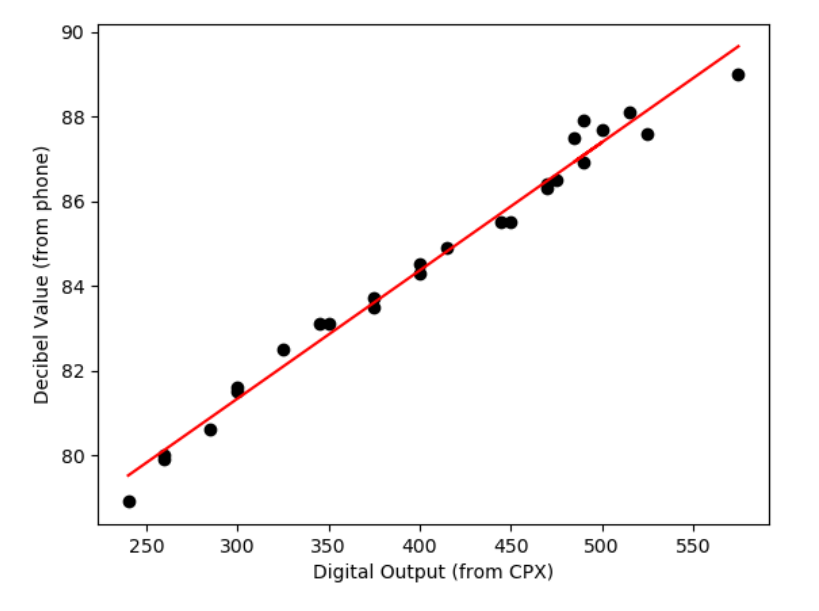
\includegraphics[height=80mm, width=100mm]{Figures/Linear_Regression.png}
  \end{center}
  \caption{Linear Regression Example}\label{f:linear_regression}
\end{figure}
In this case the ordinate axis is the output $Y$ and the abscissa is
the independent variable that characterizes the matrix ${\bf H}$. The
black dots then are the measurements $\bar{Y}$ while the trend line is
the estimate $\tilde{Y} = {\bf H}\tilde{x}$. In this case the residuals
$\hat{Y} = \tilde{Y}-\bar{Y}$ is the distance between the trend line
in red and the black dots (the measurements). For this linear example,
the unknowns would be the slope and intercept. It is clear here that
there exists no linear solution $\vec{x}$ that goes through all black
data points. Thus, the equation below can be constructed.
\begin{equation}
  \bar{Y} = {\bf H}\tilde{x} + \hat{Y}
\end{equation}
This implies that the trendline $\tilde{Y}$ would go through all data
points if $\hat{Y}$ were zero. Thus the solution to this problem was
originally found by Gauss \cite{stigler1981} and involved minimizing
the residuals between $\bar{Y}$ and $\tilde{Y}$ (the estimated Y
values). To do this, a cost function is generated such that
\begin{equation}
  J = \frac{1}{2}\hat{Y}^T \hat{Y}
\end{equation}
Substituting in the equation $\hat{Y} = \bar{Y} - {\bf H}\tilde{x}$
and minimizing the cost function $\partial J/\partial \tilde{x} = 0$
results in the solution below.
\begin{equation}
  \tilde{x} = ({\bf H}^T{\bf H})^{-1}{\bf H}^T\bar{Y}
\end{equation}
Note that the equation above only works if the number of measurements $M$
is greater than or equal to the number of unknowns $N$. If not, the
solution will always be rank deficient and no solution will be
found. This is called an under constrained problem. In this there are
an infinite number of solutions that satisfy $\bar{Y} = {\bf
  H}\vec{x}$ even in the presence of modeling errors. In order
to get around this issue Lagrange's method of 
optimization is used \cite{lagrange}. For problems like this the
residuals between the estimate $\tilde{Y}$ and the measured signals
$\bar{Y}$ can be easily made to be zero. Thus minimizing the residuals
is trivial since the solution will still be an infinite number of
solutions. Therefore a constraint can be placed where
$\bar{Y}=\tilde{Y}={\bf H}\tilde{x}$. In order to find a unique
solution then the requirement is placed to minimize the estimate
$\tilde{x}$. In this case, the cost function
to be minimized is given by Lagrange's extension to optimization as
shown below
\begin{equation}
L = \frac{1}{2}\tilde{x}^T\tilde{x} + \lambda^T(\bar{Y}-{\bf H}\tilde{x})
\end{equation}
The cost function above utilizes the method of Lagrange multipliers in
order to satisfy the constraint that the solution must pass through
all measurements again only if the number of measurements $M$ is less than
the number of unknowns $N$. In the equation above the vector
$\tilde{x}$ must be solved and so must the Lagrange multipliers
$\lambda$. The solution to the problem above requires
$\partial L / \partial \tilde{x} = 0$ and $\partial L / \partial \lambda = 0$. Carrying out the partial derivatives and solving for the estimate
yields the following equations. 
\begin{equation}
  \tilde{x} = {\bf H}^T({\bf H}{\bf H}^T)^{-1}\bar{Y}
\end{equation}
Note, it is standard practice in state estimation to have at least as
many measurements as unknowns. In this case $M=N$ and Gauss' solution
is sufficient. 

\subsection{Weighted Least Squares}

The weighted least squares solution is found by setting the cost
function equal to $J = \frac{1}{2}\hat{Y}^T{\bf W}\hat{Y}$
where {\bf W} is a positive definite and symmetric weighting matrix. The solution then is
shown below.
\begin{equation}\label{e:weights}
  \tilde{x} = ({\bf H}^T{\bf W}{\bf H})^{-1}{\bf H}^T{\bf W}\bar{Y}
\end{equation}
In the standard Kalman Filter approach, the weighting matrix is given
by the inverse covariance of the error ${\bf r} = {\bf
  E}[\vec{v}\vec{v}^T]$. Placing this into a matrix yield ${\bf W} =
{\bf R}^{-1}$ where ${\bf R} = diag([{\bf r}_1,...{\bf r}_M])$.  
The weighted least squares solution then reduces to
\begin{equation}
  \tilde{x} = ({\bf H}^T{\bf R}^{-1}{\bf H})^{-1}{\bf H}^T{\bf R}^{-1}\bar{Y}
\end{equation}

\subsection{A Priori Knowledge of the State Vector}

If a priori knowledge is obtained via other means or in the case of
the standard Kalman Filter from integration of the state, it is
possible to obtain an updated estimate of the state based on the
previous state estimate and the new sensor measurements. First, the a
priori estimate $\tilde{x}^{-}$ is written as 
\begin{equation}
  \tilde{x}^{-} = \vec{x} +  \vec{w}
\end{equation}
where $\vec{w}$ is model noise associated with the error in the
state estimate. The covariance of this noise is also denoted as a
matrix and defined below.
\begin{equation}
  cov(\vec{w}) = {\bf E}(\vec{w}\vec{w}^T) = {\bf q}
\end{equation}
In this case it is desired for the updated measurement to be some
linear combination of the a priori equation and the measurements such
that
\begin{equation}
  \tilde{x} = {\bf \Lambda}\bar{Y} + {\bf \Gamma}\tilde{x}^{-}
\end{equation}
The matrices ${\bf \Lambda}$ and ${\bf \Gamma}$ have an added constraint
which can be shown by assuming the a priori measurement is perfect
$\tilde{x}^- = \vec{x}$ and the measurements $\bar{Y} = Y = {\bf
  H}\vec{x}$. In this case, we must have the updated estimate equal
the truth signal. $\tilde{x} = \vec{x}$. Rearranging the equation above yields
\begin{equation}
  \vec{x} = {\bf \Lambda}{\bf H}\vec{x} + {\bf \Gamma}\vec{x}
\end{equation}
which means that $({\bf \Lambda}{\bf H} + {\bf \Gamma}) = {\bf I}$
Again using the method of lagrange multipliers the cost function to be
minimized is given as
\begin{equation}
  L = {\bf E}[\frac{1}{2}\hat{x}^T\hat{x} + \lambda^T({\bf I} - {\bf
    \Lambda}{\bf H} - {\bf \Gamma})]
\end{equation}
where $\hat{x} = \tilde{x} - \vec{x}$ and again {\bf E} is the
expectation operator. Remembering that {\bf q} is
the covariance of the model noise and {\bf r} is the covariance of the
measurement noise, the solution to the minimization problem is given
by the equation below. 
\begin{equation}
  \tilde{x} = ({\bf H}^T{\bf R}^{-1}{\bf H}+{\bf q}^{-1})^{-1}({\bf
    H}^T{\bf R}^{-1}\bar{Y}+{\bf q}^{-1}\tilde{x}^{-})
\end{equation}
Note that this solution assumes that ${\bf E}(\vec{w}\vec{v}^T) = 0$. Measurement and model noise are uncorrelated.

\subsection{Complimentary Filter}

Looking at the equation for the A priori knowledge it is possible to
formulate the complimentary filter. First, the measurements are
assumed to be identical to the state vector such that ${\bf h}_k = {\bf
  I}$. From here a few extremes are shown below. First, assume that the measurement error is very low such
that the $cov(\vec{\nu})<<1$ while the model noise $\vec{w}$ is very
large approaching infinity. In this case, ${\bf q}^{-1} =0$. Substituting this into the weighted apriori equation yields
\begin{equation}
  \tilde{x} = average(\bar{Y})
\end{equation}
which essentially states that the estimate completely believes the
sensor measurement. If instead we assume that the model noise is
perfect such that $cov(\vec{w})<<1$ and the sensor noise is
approaching infinity, then ${\bf R}^{-1}=0$. This yields the following equation.
\begin{equation}
  \tilde{x} = \tilde{x}^{-}
\end{equation}
Thus it can be seen that there is a sliding bar between believing the
apriori estimate or the sensor measurement. As such it is possible to
develop a much simpler filter. First a constraint is placed on {\bf q}
and {\bf R} such that
\begin{equation}
  ({\bf H}^T{\bf R}^{-1}{\bf H}+{\bf q}^{-1}) = {\bf I}
\end{equation}
This causes the update law to reduce to the following
\begin{equation}
  \tilde{x} = {\bf H}^T{\bf R}^{-1}\bar{Y}+{\bf q}^{-1}\tilde{x}^{-}
\end{equation}
If only one measurement is investigated the equation collapses to the
following.
\begin{equation}
  \tilde{x} = {\bf r}^{-1}\bar{y}+{\bf q}^{-1}\tilde{x}^{-}
\end{equation}
The constraint also collapses to
\begin{equation}
  {\bf r}^{-1}+{\bf q}^{-1} = {\bf 1}
\end{equation}
If ${\bf q}^{-1} = {\bf s}$ and ${\bf r}^{-1}={\bf 1}-{\bf s}$ the
update law simplifies to
\begin{equation}
  \tilde{x} = ({\bf 1}-{\bf s})\bar{y}+{\bf s}\tilde{x}^{-}
\end{equation}
Here it is clear that if ${\bf s} = {\bf 1}$ the new estimate will be
equal to the old estimate meaning that the sensor noise is approaching
infinite. If ${\bf s} = 0$ it means that the new estimate is equal to
the sensor measurement meaning the model noise is approaching
infinity. This is a simple crude first order filter that can be used
when only a simple understanding of covariance is known.

\subsection{Sequential Linear Estimator}

In the above two scenarios, it is assumed that all measurements from 1
to $M$ are known at the same time instant $t$ and thus the least squares estimate can be done ``all
at once". For discrete time sensors on board a spacecraft this is
not possible. For example, if we take the weighted least squares
solution assuming we have a {\it 0th} batch of measurements, the
estimate of $\tilde{x}$ would be
\begin{equation}
  \tilde{x}_0 = ({\bf h}_0^T{\bf w}_0{\bf h}_0)^{-1}{\bf h}_0^T{\bf
    w}_0\bar{y}_0
\end{equation}
If we then waited $\Delta t$ seconds for a new set of measurements we
would have to obtain a new estimate of $\tilde{x}$ which could be done
using the equation below
\begin{equation}
  \tilde{x}_1 = ({\bf h}_1^T{\bf w}_1{\bf h}_1)^{-1}{\bf h}_1^T{\bf
    w}_1\bar{y}_1
\end{equation}
This solution however would only take into account the new
measurements. Thus, if larger matrices were constructed like
${\bf H} = [{\bf h}_0,{\bf h}_1]$ the solution for $\tilde{x}$ becomes
the same as it was in Equation \ref{e:weights}. This process would be
tedious if these matrices were computed over and over again. This is
because the matrices would continue to grow larger and larger over
time and eventually overflow the memory management system on the
computer. Thus, a method for updating the state vector every time
a new measurement is obtained must be derived. To do this the two
equations are substituted into equation \ref{e:weights}. Then a
covariance matrix is used such that ${\bf p} = ({\bf h}^T{\bf w}{\bf h})^{-1}$ 
which never grows in size. Using that simplification and making use of
a estimation gain matrix ${\bf k}$, the estimation algorithm is as follows:
\begin{enumerate}[itemsep=-5pt]
    \item The first measurement is obtained $\bar{y}_0$
    \item Compute the matrix ${\bf p_0} = ({\bf h}_0^T{\bf w_0}{\bf h}_0)^{-1}$
    \item Obtain the estimate for $\tilde{x}_0 = {\bf p_0}{\bf
      h}_0^T{\bf w_0}\bar{y}_0$ (Notice that if you use the equation
      above this is the same solution as the weighted least squares estimate)
    \item Every time a new measurement, $\bar{y}_k$, is obtained use the recursive least squares update law shown in the equation below.  
\end{enumerate}
\begin{equation}
  \begin{matrix}
    {\bf k}_{k+1} = {\bf p}_{k}{\bf h}_{k+1}^T[{\bf h}_{k+1}{\bf p}_k{\bf h}_{k+1}^T+{\bf w}_k^{-1}]^{-1}\\
    {\bf p}_{k+1} = [{\bf 1} - {\bf k}_{k+1}{\bf h}_{k+1}]{\bf p}_k\\
    \tilde{x}_{k+1} = \tilde{x}_k + {\bf k}_{k+1}(\bar{y}_{k+1} - {\bf h}_{k+1}\tilde{x}_k) \\
  \end{matrix}
\end{equation}
In the special case where the weighting matrix
${\bf w}_k$ is equal to a constant ${\bf w}$ and the state vector is
directly measured such that ${\bf h}_k$ is also identity, the 
sequential linear estimator gives the following simplified steps.
\begin{enumerate}[itemsep=-5pt]
    \item The first measurement is obtained $\bar{y}_0$
    \item Compute ${\bf p}_0 = {\bf w}^{-1}$
    \item Obtain the estimate for $\tilde{x}_0 = \bar{y}_0$ (this is a fault of ${\bf h}_k$ being identity) 
    \item Every time a new measurement, $\bar{y}_k$, is obtained use the recursive least squares update law shown in the equation below.  
\end{enumerate}
\begin{equation}
  \begin{matrix}
    {\bf k}_{k+1} = {\bf p}_k[{\bf p}_k + {\bf w}^{-1}]^{-1}\\ 
    {\bf p}_{k+1} = [{\bf 1} - {\bf k}_{k+1}]{\bf p}_k\\
    \tilde{x}_{k+1} = \tilde{x}_k + {\bf k}_{k+1}(\bar{y}_{k+1} - \tilde{x}_k) \\
  \end{matrix}
\end{equation}

\subsection{The Continuous Time Complimentary Filter}

In the above section a discrete sequential least squares update law
was formulated. In that derivation it is assumed that the state
estimate is held constant in between state measurements. It is
possible however to integrate a model of the state dynamics and use
that estimate in between state measurements. The is the start of a
Kalman Filter. To formulate the Continuous Time Complimentary Filter
the dynamics of the system are written such that
\begin{equation}
  \begin{matrix}
    \dot{\vec{x}} = {\bf f}\vec{x} + {\bf g}u +{\bf m}\vec{w} \\
    \vec{y} = {\bf h}\vec{x}
  \end{matrix}
\end{equation}
where the initial conditions are $\vec{x}_0$ and $\vec{w}$ is a
modeling noise term where ${\bf E}[\vec{w}\vec{w}^T]={\bf q}$ just as
was defined in the a priori estimation section. The model dynamics are
set up such that 
\begin{equation}
  \begin{matrix}
    \dot{\tilde{x}} = \tilde{{\bf f}}\tilde{x} + \tilde{{\bf g}}u + \vec{\gamma}\\
    \tilde{y} = {\bf h}\tilde{x} \\
    \bar{y} = {\bf h}\vec{x} + \vec{v}
  \end{matrix}
\end{equation}
where again $\bar{y}$ is the state measurement and $\vec{v}$ is noise
associated with the sensor where {\bf E}$[\vec{v}\vec{v}^T]=${\bf
  r}. The term $\vec{\gamma}$ is added as a psuedo control which can
be whatever we want. The idea is for $u$ to be the control input to
drive $\vec{x} \rightarrow \vec{x}_c$ while the psuedo control is for
the observer dynamics to drive $\tilde{y} \rightarrow \bar{y}$. The
model dynamics are going to deviate in between sensor measurements so
if the observer dynamics are designed properly the estimate can
converge to the measurement. Of course, this means your estimate is
only as good as your measurement noise but it is a start. To design
the psuedo control law, measurement feedback is used in the same form
as standard unity feedback control laws such that $\vec{\gamma} =
{bf k}\hat{y}$ where $\hat{y}$ is the difference between the estimate and
the measurement. The closed loop dynamics can then be written as
\begin{equation}
  \dot{\tilde{x}} = (\tilde{{\bf f}}-{\bf k}{\bf h})\tilde{x} + \tilde{{\bf g}}u
  + {\bf k}\bar{y}
\end{equation}
Looking at this equation it's hard to see the effect of the
observer. Thus the error dynamics must be investigated where
$\hat{x}=\tilde{x}-\vec{x}$. For the simple case it is assumed that
${\bf f}=\tilde{{\bf f}}$ and ${\bf g}=\tilde{{\bf g}}$. The closed
loop error dynamics can then be written as
\begin{equation}
  \dot{\hat{x}} = ({\bf f} - {\bf k}{\bf h})\hat{x} + {\bf k}\vec{v}
\end{equation}
in this case the solution to this equation is
\begin{equation}
  \hat{x}(t) = \hat{x}_0e^{({\bf f} - {\bf k}{\bf h})t} + \vec{\eta}
\end{equation}
where the term $\vec{\eta}$ is a function of the noise term ${\bf
  k}\vec{v}$. In this case, if {\bf k} is chosen to be large, the
error dynamics will be very fast but the noise term will be very
large. If {\bf k} is chosen to be very small the error dynamics will
be slow but the error term will not be a prevalent. The issue with
this filter of course comes with how to tune the gain matrix {\bf k}
which is what the Kalman filter seeks to address.
    
\subsection{The Continuous Discrete Kalman Filter}

In the case of the continuous discrete Kalman Filter, the model
dynamics are integrated just as in the complimentary filter. The only
difference is instead of using a continuous observer the state
estimate is updated every time a new measurement is obtained much like
the sequential least squares technique. First, let's write the model
dynamics as before without the observer and the measurement equations
are written such that the measurement is taken at timestep $t_k$ and
thereafter every $\Delta t$. 
\begin{equation}\label{e:model_dynamics}
  \begin{matrix}
    \dot{\tilde{x}} = \tilde{{\bf f}}\tilde{x} + \tilde{{\bf g}}u \\
    \tilde{y} = {\bf h}\tilde{x} \\
    \bar{y}_k = {\bf h_k}\vec{x}(t_k) + \vec{v}_k
  \end{matrix}
\end{equation}
The update equation is written using the continuous observer dynamics
used for the complimentary filter only in this case the update is
discrete.
\begin{equation}\label{e:state_update}
  \tilde{x}_k^+ = \tilde{x}_k^- + {\bf k}_k(\bar{y}_k-{\bf
    h_k}\tilde{x}_k^-)
\end{equation}
In this case $\tilde{x}_k^+$ is the estimated state after the update
while $\tilde{x}_k^-$ is the estimate before the update. The equation
for the covariance update and the Kalman Gain matrix are identical in
that the derivation is formulated just as it was before. The equations
are shown below again only $+$ and $-$ is used to denote the matrices
before and after update.
\begin{equation}\label{e:kalman_gain}
  \begin{matrix}
  {\bf k}_{k} = {\bf p}_{k}{\bf h}_{k}^T[{\bf h}_{k}{\bf p}_k^-{\bf h}_{k}^T+{\bf r}]^{-1}\\
  {\bf p}_{k}^+ = [{\bf 1} - {\bf k}_{k}{\bf h}_{k}]{\bf p}_k^-
  \end{matrix}
\end{equation}
In the sequential linear estimator however, the covariance matrix was
set using a weighted least squares approach. In this case the
covariance matrix is set such that ${\bf p} = {\bf
  E}[\hat{x}\hat{x}^T]$. Taking a derivative of this equation and
substituting in the closed loop error dynamics yields the covariance
propagation equation shown below.
\begin{equation}\label{e:covariance_dynamics}
  \dot{{\bf p}} = \tilde{{\bf f}}{\bf p} + {\bf p}\tilde{{\bf f}}^T +
      {\bf m}{\bf q}{\bf m}^T
\end{equation}
The final Continuous Discrete Kalman Filter then goes like this.
\begin{enumerate}
  \item Integrate the model dynamics in Equation
    \ref{e:model_dynamics} and the covariance dynamics in equation
    \ref{e:covariance_dynamics}
  \item When a measurement is received, the Kalman Gain matrix is
    computed using equation \ref{e:kalman_gain}. 
  \item Equation \ref{e:kalman_gain} is also used to update the
    covariance matrix
  \item Finally, equation \ref{e:state_update} is used to update the
    state vector estimate and then the process repeats.
\end{enumerate}
An example figure is shown below for a first order system. In this
figure the blue stars represent discrete sensor measurements with some
noise. Everytime the sensor is updated the model performs and update
and instantaneously changes to a new value. The model then integrates
(incorrectly due to model mismatch) until a new sensor measurement is
obtained. In this case the model is so inaccurate it makes more sense
to update the sensor more frequently or perform some sort of adaptive
control algorithm to estimate the plant dynamics.
\begin{figure}[H]
  \begin{center}
    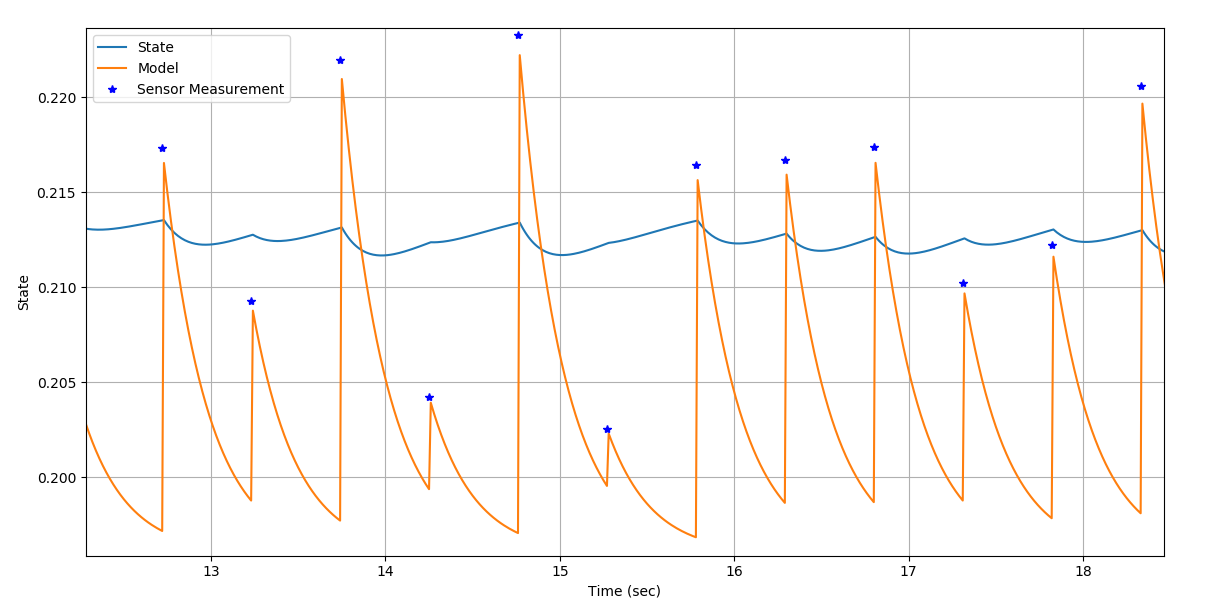
\includegraphics[height=80mm, width=140mm]{Figures/Kalman_Filter_Example.png}
  \end{center}
  \caption{First Order Kalman Filter Example}\label{f:kalman}
\end{figure}
    
\subsection{Kalman Filter for Spacecraft Dynamics}

Attitude estimation involves a combination of attitude determination
and state estimation. Assuming at time $t=t_0$ the attitude estimation
algorithm is performed and an estimate of the quaternion is obtained
as $\tilde{q}_0$. If discrete regular angular velocity
($\bar{\omega}_{k}$) measurements are made every $\Delta t$ seconds,
the quaternion can be estimated by simply integrating the attitude
equations of motion. Even if perfect sensor measurements are made, it
is possible to integrate these equations of motion over time and the
quaternion $\vec{q}$ will be much different than the estimated
quaternion $\tilde{q}$. Thus, the attitude estimation algorithm can
run again to obtain a new absolute quaternion measurement. The
equations of motion are integrated and when a new sensor measurement
is obtained the estimated state is updated based on the estimated
covariance combined with and estimate of model errors and sensor
errors. Finally, it is possible to 
create an Extended State Kalman Filter (EKF) which can estimate
sensor inaccuracies simply by finding the least squares solution
between the sensor measurements and state estimates. The sections that
follow details the Kalman Filter for Spacecraft Dynamics as well as
the extended state version which estimate bias values in the rate gyro.
  
First, the 4-dimensionality of the quaternion renders the
above Kalman filter formulation to be impossible mostly because the
quaternion derivative is a 4 by 1 matrix while the angular velocity
vector is a 3 by 1. Furthermore, the quaternion derivative is not
linear and cannot be expressed as the linear matrices in the previous
section. As such the Kalman Filter must be updated somewhat. The
derivative of the state $\dot{\vec{q}}$ is cumbersome and follows the
reference in \cite{Liu_Estimation}. First the angular 
velocity measurement is substituted into the derivative of
quaternions where the ${\bf \Omega}()$ and ${\bf \chi}()$ identity is used to
separate out the white noise parameter.
\begin{equation}
  \dot{\vec{q}} = \frac{1}{2}{\bf \Omega}(\vec{\omega})\vec{q} =
  \frac{1}{2}{\bf \Omega}(\bar{\omega}-\vec{b}-\vec{\eta}_g)\vec{q} =
  \frac{1}{2}{\bf \Omega}(\bar{\omega}-\vec{b})\vec{q} - \frac{1}{2}{\bf \chi}(\vec{q})\vec{\eta}_g
\end{equation}
At this point an error quaternion is created using the difference
between $\vec{q}$ and $\tilde{q}$. Recall that the error quaternion is
given by the equation below. The full equation is shown in
\ref{e:quat_difference}. 
\begin{equation}
  \delta \vec{q} = \vec{q}~\Earth~\tilde{q}^{-1}
\end{equation}
The derivative of this difference quaternion is beyond the scope of
this report but can be found in \cite{kalman_quat}.
\begin{equation}
  \dot{\delta \vec{q}} = \begin{Bmatrix} 0 \\ -{\bf
      S}(\tilde{\omega})\delta \vec{\epsilon} \end{Bmatrix} +
  \frac{1}{2}{\bf \Omega}(\delta \vec{\omega})\delta \vec{q}
\end{equation}
where $\delta \vec{\omega} = \vec{\omega} - \tilde{\omega}$ and
$\delta \vec{\epsilon} = \vec{\epsilon} - \tilde{\epsilon}$. Recall
that $\tilde{\omega} = \bar{\omega}-\tilde{b}$. The second term in the
equation above can be expanded using the equations in Section
\ref{s:measurements}. Note that $\delta \vec{\omega}$ simplifies to
$-\delta \vec{b} - \vec{\eta}_g$ and $\dot{\delta \vec{q}} = [\dot{\delta q_0},\dot{\delta
    \vec{\epsilon}}]^T$. 
\begin{equation}
  \dot{\delta \vec{q}} = \begin{Bmatrix} 0 \\ -{\bf
      S}(\tilde{\omega})\delta \vec{\epsilon} \end{Bmatrix} -
  \frac{1}{2}\begin{Bmatrix} -\delta \vec{\epsilon}^T\delta \vec{b}
    \\ \delta q_0 \delta \vec{b} + {\bf S}(\delta
    \vec{\epsilon})\delta \vec{b} \end{Bmatrix} -
  \frac{1}{2}\begin{Bmatrix} -\delta \vec{\epsilon} \vec{\eta}_g
    \\ \delta q_0 \vec{\eta}_g + {\bf S}(\delta
    \vec{\epsilon})\vec{\eta}_g \end{Bmatrix}
\end{equation}
In order to proceed further, small angle
approximations are made such that $|\delta \vec{q}|<<1$. The latter 3
variables in the quaternion are further approximated as $\delta
\vec{\rho} = \delta \vec{\epsilon}$. In order to fit in with the standard
Kalman filter, the state vector $\vec{x} = \vec{\rho}$ and thus the state
dynamics $\dot{\delta \vec{x}}$ can then be written as
\begin{equation}
  \dot{\delta \vec{x}} = \dot{\delta \vec{\rho}} = -{\bf
    S}(\tilde{\omega})\delta \vec{d} - \frac{1}{2}\delta \vec{b} -
  \frac{1}{2}\vec{\eta}_g
\end{equation}
In order to extract the attitude quaternion from the approximated
state the following equations are used.
\begin{equation}
  \begin{matrix}
    \delta \vec{\epsilon} = \frac{\delta \vec{\rho}}{\sqrt{1+\delta
        \vec{\rho}^T\delta \vec{\rho}}} & q_0 = \frac{1}{\sqrt{1+\delta
        \vec{\rho}^T\delta \vec{\rho}}}
  \end{matrix}
\end{equation}

\subsection{Extended State Kalman Filter}

As shown in the previous section, a Kalman filter can be used to
estimate the state. The standard Kalman filter however can be extended
to include the bias of the angular velocity measurement. Thus the
state vector is augmented to be $\vec{x} = [\vec{q},\vec{b}]^T$. Since
the derivative of the bias is the white noise vector, the difference
state vector after much simplification is shown below.
\begin{equation}
  \dot{\delta \vec{x}} = \begin{Bmatrix} \dot{\delta \vec{\rho}}
    \\ \delta \vec{b} \end{Bmatrix} =
  \begin{bmatrix} -{\bf S}(\tilde{\omega}) & -\frac{1}{2}{\bf I}_{3x3} \\
    {\bf 0}_{3x3} & {\bf 0}_{3x3} \end{bmatrix}
  \begin{Bmatrix} \delta \vec{\rho} \\\delta \vec{b} \end{Bmatrix} +
  \begin{Bmatrix} -\frac{1}{2}\vec{\eta}_g \\ \vec{\eta}_b \end{Bmatrix}
\end{equation}
In this formulation $\delta \vec{b} = \vec{b} - \tilde{b}$. The
derivative is then $\delta \dot{\vec{b}} = \vec{\eta}_b - 0$. It is
assumed that the derivative of the estimate is zero and thus is only
updated when sensor measurements are made. The states equation above can be
reduced to the state space form shown below. 
\begin{equation}
  \dot{\delta \vec{x}} = {\bf A}\delta \vec{x} + \vec{\eta}
  \end{equation}

%%%%%%%%%%%%%%%%%%%%%%%%%%%%%%%%%%%%%%%%%%%%%%%%%%%%%%%%%%%%%%%%%%%

\bibliographystyle{unsrt}
\bibliography{papers.bib}

\end{document}
